\documentclass[14pt, a4paper]{extarticle}
\usepackage[russian]{babel}
\usepackage{indentfirst}
\usepackage{setspace}
\usepackage{geometry}
\usepackage{caption}
\usepackage{graphicx}
\usepackage{chngcntr}
\usepackage{float}
\usepackage{url}
\usepackage[protrusion=false]{microtype}   % отключаем protrusion для TU-кодировки
\usepackage{tabularx}

\usepackage{tempora}                        % Times New Roman для кириллицы (работает в XeLaTeX)
\usepackage[bigdelims,vvarbb]{newtxmath}
\usepackage[cal=boondoxo]{mathalfa}

\usepackage{longtable}
\usepackage{xltabular}
\usepackage{ragged2e}
\newcolumntype{L}{>{\RaggedRight\arraybackslash}X}

\babelfont[russian]{rm}[
Scale=MatchUppercase,
ItalicFont={Tempora-Italic.otf},
BoldFont={Tempora-Bold.otf},
BoldItalicFont={Tempora-BoldItalic.otf}
]{Tempora-Regular.otf}

% Рисунки
\counterwithin{figure}{section}

\captionsetup[figure]{
	labelsep=endash,
	name={Рисунок}
}

\setlength{\intextsep}{1\baselineskip}

% Отступы
\geometry{left=3cm, right=1.5cm, top=2cm, bottom=2cm}
\onehalfspacing
\setlength{\parindent}{1.25cm}
\setlength{\parskip}{0pt}

% Таблицы
\captionsetup[table]{
	justification=raggedright,
	singlelinecheck=false,
	labelsep=space,
	skip=4pt
}

% Разделы
\makeatletter
%\renewcommand\section{\@startsection{section}{1}{1.25cm}%
%	{-3.5ex \@plus -1ex \@minus -.2ex}%
%	{2.3ex \@plus.2ex}%
%	{
%		\ctearpage
%		\bfseries
%		\fontsize{16}{1.5}\selectfont
%}}


\renewcommand\section{\clearpage\@startsection{section}{1}{1.25cm}%
	{-3.5ex \@plus -1ex \@minus -.2ex}%
	{2.3ex \@plus.2ex}%
	{%
		\bfseries
		\fontsize{16}{1.5}\selectfont
}}

\renewcommand{\thesection}{\arabic{section}}
\renewcommand{\@seccntformat}[1]{\csname the#1\endcsname\space}
\makeatother

\begin{document}
	\begin{titlepage}
		\centering
		Министерство науки и высшего образования Российской Федерации
		
		Федеральное государственное автономное образовательное учреждение высшего образования
		
		\MakeUppercase{Томский}
		
		\vspace{1\baselineskip}
		
		Кафедра
		
		\vspace{2\baselineskip}
		
		{\bfseries\MakeUppercase{
			Разработка адаптивной системы управления двигателем с нейросетевой обработкой данных
		}}
		
		Отчет по разработке по дисциплине "системная инженерия"
		
		\vspace{1\baselineskip}
		
		\begin{flushright}
			Студент гр. 956-М:
			
			{\rule{1.5cm}{0.4pt} Д. И. Цымбалов}
			
			"\rule{1.5cm}{0.4pt}" \rule{2cm}{0.4pt} {\the\year}г.
			
			\vspace*{1\baselineskip}
			
			Проверил:
			
			Должность (Доцент кафедры ПрЭ):
			
			{\rule{1.5cm}{0.4pt} А. С. Королев}
			
		\end{flushright}
		
		\vfill
		{Томск \the\year}
		
	\end{titlepage}
	
	\section{Контекст деятельности}
		Контекст деятельности: процесс управления двигателем внутреннего сгорания (ДВС) в составе автомобиля
		
		Участники процесса:
		
		\begin{itemize}
			\item Водитель — задаёт режим (педаль, нагрузки);
			\item Сервисный инженер/диагност — читает DTC, логи, версии модели.
			\item OEM-инженер — отвечает за калибровки и обновления.
			\item Регулятор (экология) — задаёт нормативы.
			\item Поставщик ЭБУ/полупроводников — обеспечивает платформу и вычислительные ресурсы.
		\end{itemize}
	
		\subsection{Декомпозиция процесса деятельности}
		
		
		Текущий процесс (AS-IS) — статическая калибровка ЭБУ
		
		\begin{enumerate}
			\item Подготовка
			
			\begin{enumerate}
				\item Стендовые калибровки под «усреднённый» двигатель и топливо;
				\item прошивка статических таблиц в ЭБУ;
				\item cертификация на цикле;
				\item уастройка порогов DTC;
			\end{enumerate}
			
			\item Эксплуатация
			\begin{enumerate}
				\item Считывание датчиков
				\item Выбор калибровки по таблице «нагрузка/обороты»
				\item Формирование воздействий
				\item Контроль по лямбде/детонации без изменения коэффициентов
				
			\end{enumerate}
			
			\item Обслуживание
			\begin{enumerate}
				\item Периодическое чтение DTC
				\item Ручная корректировка при ремонте;
				\item Документирование;
			\end{enumerate}
			
		\end{enumerate}
		
		Проблемные зоны AS-IS: таблицы не адаптируются к износу, топливу, климату; нет динамической коррекции по ходу движения; риск детонации; ложные DTC; ручные правки.
		
		\subsubsection{Целевой процесс (TO-BE) — динамическая ИИ-калибровка ЭБУ по ходу движения}
		
			Основной процесс: «Адаптивное управление ДВС с динамической коррекцией калибровочных коэффициентов ИИ-модулем в реальном времени по ходу движения».
		
		\begin{enumerate}
			\item Сбор данных (непрерывно, по ходу движения);
			\begin{enumerate}
				\item Приём сигналов датчиков (ДМРВ/ДАД, лямбда, ДПКВ, ДПРВ, детонация, t° ОЖ/воздуха, давление топлива) с частотой ≥100 Гц;
				\item Валидация диапазонов и достоверности;
			\end{enumerate}
			
			\item Оценка состояния (в реальном времени);
			\begin{enumerate}
				\item Расчёт текущего режима (нагрузка/обороты);
				\item Детекция аномалий (детонация, пропуски, обеднение/обогащение);
			\end{enumerate}
			
			\item Динамическая ИИ-коррекция коэффициентов;
			\begin{enumerate}
				\item ИИ-инференс на борту: расчёт поправок $\Delta$-коэффициентов (топливо, УОЗ, наддув, EGR) по текущим данным, без остановки движения;
				\item Валидация поправок в безопасных пределах (ограничения по детонации/ресурсу);
				\item Динамическое обновление коэффициентов с логированием каждого действия;
			\end{enumerate}
			
			\item Контроль результата;
			\begin{enumerate}
				\item Обратная связь по лямбде, детонации, мощности/расходу;
				\item Оценка эффективности коррекции;
				\item Решение о продолжении/откате;
			\end{enumerate}
			
			\item Диагностика и логирование;
			\begin{enumerate}
				\item DTC, логи, телеметрия;
				\item Откат к базовым калибровкам при небезопасной коррекции (limp-home);
				\item Передача в OBD-II/облако;
			\end{enumerate}
		\end{enumerate}
		
		Ключевое отличие TO-BE: коэффициенты ЭБУ корректируются динамически по ходу движения, а не выбираются из статической таблицы; ИИ-модуль работает в замкнутом контуре с валидацией и откатом.
		
		\vspace{\parindent}
		\noindent
		\begin{minipage}{\textwidth}
			\captionof{table}{Заинтересованные стороны}
			\label{tab:stakeholders}
			\begin{tabularx}{\textwidth}{|c|X|c|}
				\hline
				\textbf{Id} & \textbf{Заинтересованная сторона} & \textbf{Приоритет} \\
				\hline
				St.01 & Автовладелец & Высокий \\
				\hline
				St.02 & Автопроизводитель (OEM) & Высокий \\
				\hline
				St.03 & Сервис/диагност & Средний \\
				\hline
				St.04 & Регулятор (экология) & Средний \\
				\hline
				St.05 & Поставщик ЭБУ/полупроводников & Низкий \\
				\hline
			\end{tabularx}
		\end{minipage}
		\vspace{\parindent}
		
		
		
		\vspace{\parindent}
		\noindent
		\begin{minipage}{\textwidth}
			\captionof{table}{Целевые показатели удовлетворения интересов заинтересованных сторон}
			\label{tab:problems}
			\begin{tabularx}{\textwidth}{|c|X|c|}
				\hline
				\textbf{Id} & \textbf{Проблема} & \textbf{Трассировка} \\
				\hline
				Pr.01 & Статические калибровки не адаптируются к износу/топливу → рост расхода и выбросов & St.01, St.02 \\
				\hline
				Pr.02 & Детонация и переобеднение при некачественном топливе → риск ресурсу & St.01, St.02 \\
				\hline
				Pr.03 & Ложные/пропущенные DTC → лишние визиты в сервис & St.01, St.03 \\
				\hline
				Pr.04 & Ручная корректировка калибровок при ремонте → время и ошибки & St.03, St.02 \\
				\hline
				Pr.05 & Нет прозрачного лога коррекций → сложно доказать соответствие нормам & St.04, St.02 \\
				\hline
			\end{tabularx}
		\end{minipage}
		\vspace{\parindent}
		
		
		\vspace{\parindent}
		\noindent
		\begin{minipage}{\textwidth}
			\captionof{table}{Потребности заинтересованных сторон}
			\label{tab:needs}
			\begin{tabularx}{\textwidth}{|c|X|c|}
				\hline
				\textbf{ID} & \textbf{Потребность} & \textbf{Трассировка} \\
				\hline
				N.01 & Снизить расход топлива при сохранении динамики за счёт динамической ИИ-коррекции по ходу движения & Pr.01 \\
				\hline
				N.02 & Исключить детонацию и опасные режимы за счёт адаптивной коррекции УОЗ/наддува в реальном времени & Pr.02 \\
				\hline
				N.03 & Сократить ложные DTC и время диагностики благодаря адаптивным порогам и прозрачным логам & Pr.03 \\
				\hline
				N.04 & Автоматизировать динамическую корректировку калибровочных коэффициентов ЭБУ без остановки движения & Pr.04 \\
				\hline
				N.05 & Обеспечить прослеживаемость коррекций (аудит-трейс) для регулятора и OEM & Pr.05 \\
				\hline
			\end{tabularx}
		\end{minipage}
		\vspace{\parindent}
		
		
		\vspace{\parindent}
		\noindent
		\begin{minipage}{\textwidth}
			\captionof{table}{Цели заинтересованных сторон}
			\label{tab:goals}
			\begin{tabularx}{\textwidth}{|c|X|c|}
				\hline
				ID & Цель & Трассировка \\
				\hline
				G.01 & Снизить средний расход топлива на 3--5\% без роста числа DTC за счёт динамической ИИ-коррекции & N.01 \\
				\hline
				G.02 & Обеспечить 0 опасных детонационных событий на 10\,000 км за счёт коррекции в реальном времени & N.02 \\
				\hline
				G.03 & Сократить ложные DTC до \(\leq 1\) на 10\,000 км & N.03 \\
				\hline
				G.04 & Автоматизировать 100\% динамических коррекций с логированием и откатом & N.04 \\
				\hline
				G.05 & Обеспечить 100\% прослеживаемость коррекций (аудит-трейс) & N.05 \\
				\hline
			\end{tabularx}
		\end{minipage}
		\vspace{\parindent}
		
		
		\vspace{\parindent}
		\noindent
		\begin{minipage}{\textwidth}
			\captionof{table}{Целевые показатели удовлетворения интересов заинтересованных сторон}
			\label{tab:targets}
			\begin{tabularx}{\textwidth}{|c|X|c|}
				\hline
				ID & Показатель удовлетворённости & Трассировка (ЗС \(\to\) цель) \\
				\hline
				StG.01 & \(\Delta\) расхода топлива \(-3\ldots-5\%\) при сохранении динамики & St.01 \(\to\) G.01 \\
				\hline
				StG.02 & 0 опасных детонаций на 10\,000 км & St.01 \(\to\) G.02 \\
				\hline
				StG.03 & Ложные DTC \(\leq 1\) на 10\,000 км & St.03 \(\to\) G.03 \\
				\hline
				StG.04 & 100\% динамических коррекций логируются и обратимы & St.03 \(\to\) G.04 \\
				\hline
				StG.05 & 100\% циклов с аудит-трейсом коррекций & St.04 \(\to\) G.05 \\
				\hline
				StG.06 & Доля циклов в норме по выбросам \(\geq 99{,}5\%\) & St.02 \(\to\) G.01/G.05 \\
				\hline
			\end{tabularx}
		\end{minipage}
	
	
	\section{Определение целевой системы}
	Для решения выявленных проблем (Pr.01–Pr.05), связанных с отсутствием адаптации калибровок ЭБУ к реальным условиям эксплуатации, ростом расхода/выбросов, риском детонации и непрозрачной диагностикой, был проведён системный анализ альтернативных вариантов. В основе выбора лежит метод взвешенных сумм, позволяющий объективно сравнить варианты с учётом приоритетов заинтересованных сторон и стратегических целей надсистемы (G.01–G.05).
	
	
	\begin{figure}[H]
		\centering
		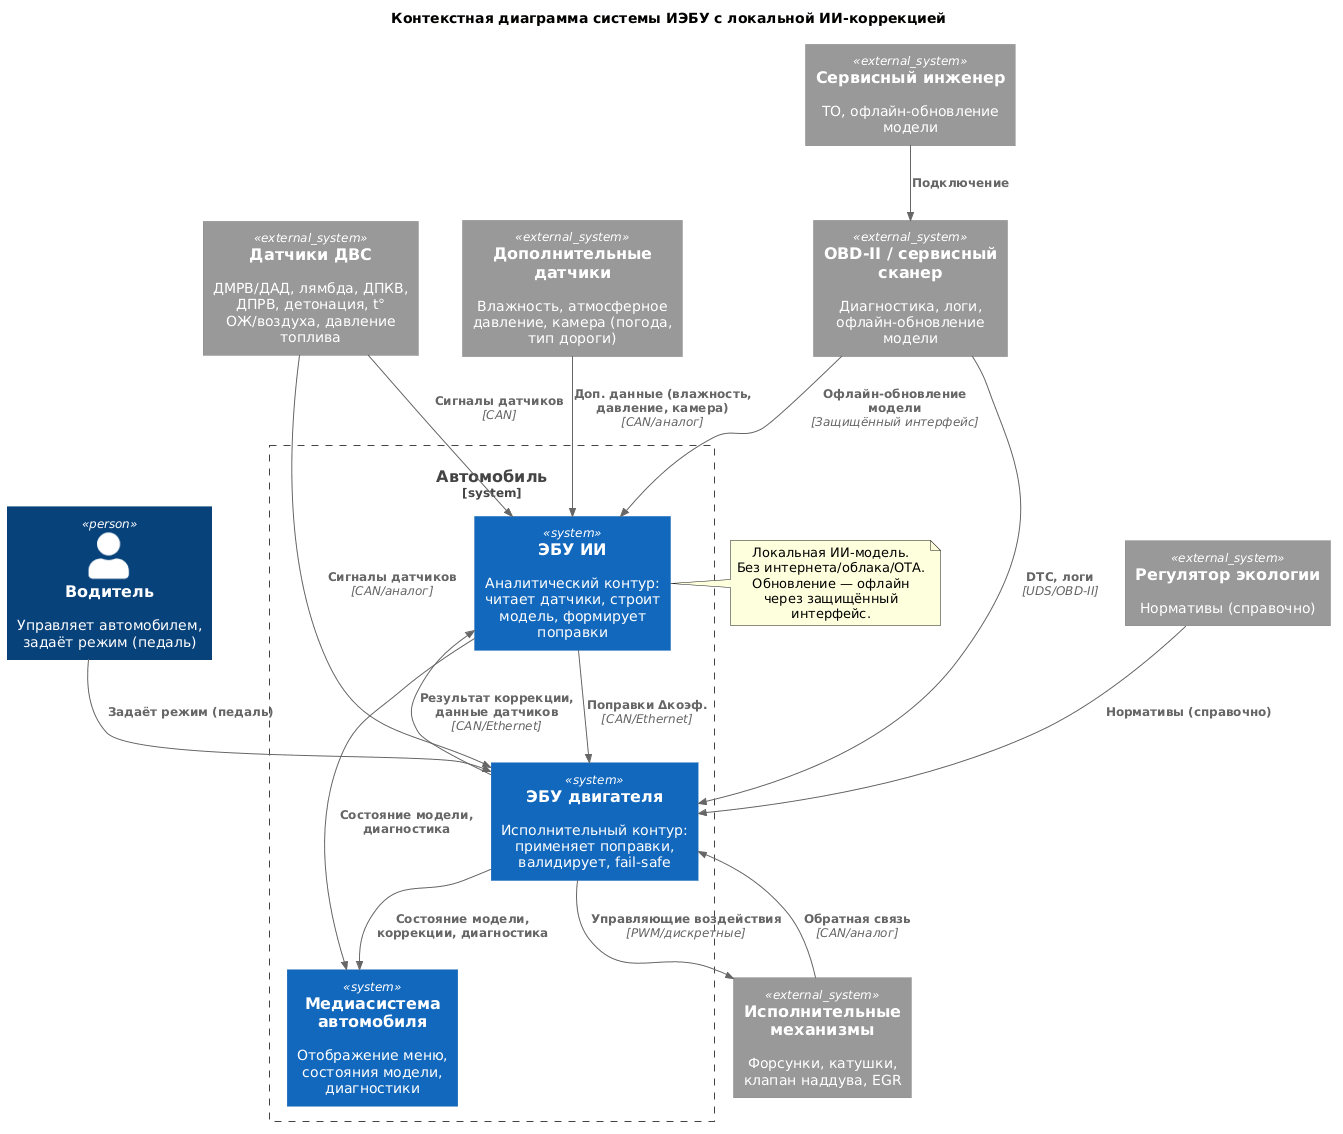
\includegraphics[width=1\linewidth]{pic/wObFAhTers.png}
		\caption{Диаграмма последовательности}
		\label{fig:p1}
	\end{figure}
	
	
	\subsection{Генерация вариантов решения}
	На этапе генерации альтернатив были рассмотрены решения в нескольких измерениях — от минимальных изменений в существующем процессе до полной технологической трансформации:
	\begin{itemize}
		\item Организационные меры (V1) — повышение квалификации персонала и регламентная ручная корректировка калибровок. Снижает ошибки, но не решает проблему адаптации в реальном времени.
		
		\item Инженерно-технические решения на уровне производства (V2, V3) — модернизация стендового оборудования и инфраструктуры калибровки. Снижает погрешность статических таблиц, но требует капиталовложений и не обеспечивает динамику по ходу движения.
		
		\item Автоматизация процессов (V4, V5) — от частичной автоматизации до комплексного решения (гибрид: бортовой ИИ + облачное дообучение)
	\end{itemize}
	
	Выбор пяти вариантов обеспечил достаточное покрытие спектра возможных решений. Каждый вариант анализировался с позиции его способности решить поставленные проблемы (Pr.01–Pr.05) и достичь целей (G.01–G.05), определённых в п.1.
	
	\vspace{\parindent}
	\noindent
	\begin{minipage}{\textwidth}
		\captionof{table}{Варианты решения обозначенной проблемы}
		\label{tab:variants}
		\begin{tabularx}{\textwidth}{|c|X|X|}
			\hline
			\textbf{№} & \textbf{Вариант} & \textbf{Краткое описание} \\
			\hline
			V1 & Табличная адаптация (без ИИ) & Классические коррекции по лямбде/детонации; калибровки остаются статическими, корректируются только пороги \\
			\hline
			V2 & Модернизация стендового оборудования & Повышение точности стендовых калибровок; не решает проблему адаптации по ходу движения \\
			\hline
			V3 & Модернизация инфраструктуры калибровки & Единая среда калибровок и версионирования; статика сохраняется, но снижается время обновления \\
			\hline
			V4 & Бортовой ИИ-модуль & Лёгкая нейросеть/регрессия на борту ЭБУ; динамическая коррекция по ходу движения, но без дообучения \\
			\hline
		\end{tabularx}
	\end{minipage}
	\vspace{\parindent}
	
		
	\subsection{Формирование системы критериев оценки}
	Система критериев (таблица 7) сформирована на основе приоритетов заинтересованных сторон и стратегических целей:
	
	\begin{itemize}
		\item K1–K3 (эффективность решения проблем) — критерии, напрямую связанные с достижением целей G.01–G.03. Имеют наибольший вес (0.60 в сумме), что отражает первостепенную важность решения исходных проблем.
		\item K4–K5 (экономическая эффективность) — стоимость и окупаемость, обеспечивают бизнес-обоснование решения.
		\item K6–K7 (эксплуатационные характеристики) — надёжность и соответствие требованиям, гарантируют долгосрочную работоспособность.
		\item K8 (локальность/security) — отсутствие внешних каналов, работа без интернета. Вес добавляется отдельно, так как это жёсткое требование.
	\end{itemize}
	
	\vspace{\parindent}
	\noindent
	\begin{xltabular}{\textwidth}{|c|L|L|L|}
		\caption{Критерии оценки вариантов}\label{tab:criteria}\\
		\hline
		\textbf{ID} & \textbf{Критерий} & \textbf{Описание} & \textbf{Шкала (1–10)} \\
		\hline
		\endfirsthead
		% шапка на последующих страницах
		\hline
		\textbf{ID} & \textbf{Критерий} & \textbf{Описание} & \textbf{Шкала (1–10)} \\
		\hline
		\endhead
		% подвал (необязательно)
		\hline
		\endfoot
		\hline
		\endlastfoot
		% --- данные ---
		K1 & Безопасность (fail-safe, откат) & Исключение опасных режимов, гарантированный откат при аномалии (G.02) & 1 (нет отката) — 10 (100\% откат) \\
		\hline
		K2 & Задержка реакции (real-time) & Время от входа датчика до воздействия (G.01) & 1 (>100 мс) — 10 (≤10 мс) \\
		\hline
		K3 & Точность коррекции / эффективность & Отклонение от оптимума, снижение расхода/выбросов (G.01, G.05) & 1 (>10\%) — 10 (≤2\%) \\
		\hline
		K4 & Стоимость и вычислительные ресурсы (инверсный) & Капитальные затраты, бюджет ЭБУ (G.04) & 1 (очень дорого) — 10 (дёшево) \\
		\hline
		K5 & Maintainability / обновляемость & OTA, версионирование, время локализации (G.03, G.04) & 1 (>1 ч) — 10 (≤5 мин) \\
		\hline
		K6 & Надёжность и обслуживаемость & MTBF, трудозатраты на ТО (G.02) & 1 (частые отказы) — 10 (редкие отказы) \\
		\hline
		K7 & Соответствие регуляторным требованиям & ISO 26262, ISO 21448, Евро-6/7 (G.05) & 1 (частичное) — 10 (полное, с аудит-трейсом) \\
		\hline
		K8 & Локальность / Security & Отсутствие внешних каналов, работа без интернета, защита от вмешательства & 1 (зависит от сети) — 10 (полностью автономно) \\
		\hline
	\end{xltabular}
	\vspace{\parindent}

	\subsection{Определение значимости критериев}
	
	Веса критериев (таблица \ref{tab:weights}) определены на основе приоритетов ЗС и стратегической важности целей:
	\begin{itemize}
		\item K1 «Безопасность» — 0.22 (критично для St.01, St.02; ISO 26262/21448).
		\item K2 «Задержка» — 0.18 (динамическая коррекция по ходу движения).
		\item K3 «Точность» — 0.13 (расход/выбросы).
		\item K4 «Стоимость» — 0.10.
		\item K5 «Maintainability» — 0.09.
		\item K6 «Надёжность» — 0.09.
		\item K7 «Соответствие нормам» — 0.09.
		\item K8 «Локальность/Security» — 0.10 (жёсткое требование, но не доминирует над безопасностью; при равенстве — приоритет у K8).
	\end{itemize}
	
	Суммарный вес критериев эффективности решения проблем (K1–K3) составляет 0.53, что подчёркивает фокус на решении исходных проблем, а не только на экономических или технических аспектах.


	\vspace{\parindent}
	\noindent
	\begin{xltabular}{\textwidth}{|c|L|L|c|}
		\caption{Значимость критериев}\label{tab:weights}\\
		\hline
		\textbf{Критерий} & \textbf{Обоснование веса} & \textbf{Вес (Σ=1)} \\
		\hline
		\endfirsthead
		% шапка на последующих страницах
		\hline
		\textbf{Критерий} & \textbf{Обоснование веса} & \textbf{Вес (Σ=1)} \\
		\hline
		\endhead
		% подвал (необязательно)
		\hline
		\endfoot
		\hline
		\endlastfoot
		% --- данные ---
		K1 & Критичен для St.01 и St.02 (ISO 26262/21448) 
		$\rightarrow$ G.02 & 0.22 \\
		\hline
		K2 & Критичен для динамической коррекции по ходу движения 
		$\rightarrow$ G.01 & 0.18 \\
		\hline
		K3 & Влияет на расход/выбросы 
		$\rightarrow$ G.01, G.05 & 0.13 \\
		\hline
		K4 & Бюджетные ограничения важны, но вторичны & 0.10 \\
		\hline
		K5 & Офлайн-обновление и локализация аномалии 
		$\rightarrow$ G.03 & 0.09 \\
		\hline
		K6 & Влияет на долгосрочную эксплуатацию & 0.09 \\
		\hline
		K7 & Юридические риски 
		$\rightarrow$ G.05 & 0.09 \\
		\hline
		K8 & Локальность/Security — обязательное требование & 0.10 \\
		\hline
		\textbf{Σ} & & \textbf{1.00} \\
		\hline
	\end{xltabular}
	\vspace{\parindent}	

	\subsection{Оценка вариантов и выбор оптимального решения}
		Оценка проводилась методом взвешенных сумм: $Score = \sum (\text{вес}_i \cdot \text{оценка}_i)$. Результаты — в таблице \ref{tab:scores}.
		
		\vspace{\parindent}
		\noindent
		\begin{xltabular}{\textwidth}{|c|L|L|L|L|L|L|L|L|L|}
			\caption{Оценка вариантов по критериям}\label{tab:scores}\\
			\hline
			\textbf{Вариант} & \textbf{K1 (0.22)} & \textbf{K2 (0.18)} & \textbf{K3 (0.13)} & \textbf{K4 (0.10)} & \textbf{K5 (0.09)} & \textbf{K6 (0.09)} & \textbf{K7 (0.09)} & \textbf{K8 (0.10)} & \textbf{Итог} \\
			\hline
			\endfirsthead
			% шапка на последующих страницах
			\hline
			\textbf{Вариант} & \textbf{K1 (0.22)} & \textbf{K2 (0.18)} & \textbf{K3 (0.13)} & \textbf{K4 (0.10)} & \textbf{K5 (0.09)} & \textbf{K6 (0.09)} & \textbf{K7 (0.09)} & \textbf{K8 (0.10)} & \textbf{Итог} \\
			\hline
			\endhead
			% подвал (необязательно)
			\hline
			\endfoot
			\hline
			\endlastfoot
			% --- данные ---
			V1 & 9 & 9 & 5 & 9 & 6 & 8 & 7 & 10 & 7.85 \\
			\hline
			V2 & 8 & 7 & 6 & 6 & 5 & 7 & 7 & 10 & 7.00 \\
			\hline
			V3 & 8 & 7 & 6 & 6 & 8 & 7 & 8 & 10 & 7.35 \\
			\hline
			V4 & 9 & 9 & 9 & 7 & 8 & 8 & 9 & 10 & \textbf{8.65} \\
			\hline
		\end{xltabular}
		\vspace{\parindent}
	
		Расчёт итоговых оценок
		$$V1 = 0.22 \cdot 9 + 0.18 \cdot 9 + 0.13 \cdot 5 + 0.10 \cdot 9 + 0.09 \cdot 6 + 0.09 \cdot 8 + 0.09 \cdot 7 + 0.10 \cdot 10 = 7.85$$
		$$V2 = 0.22 \cdot 8 + 0.18 \cdot 7 + 0.13 \cdot 6 + 0.10 \cdot 6 + 0.09 \cdot 5 + 0.09 \cdot 7 + 0.09 \cdot 7 + 0.10 \cdot 10 = 7.00$$
		$$V3 = 0.22 \cdot 8 + 0.18 \cdot 7 + 0.13 \cdot 6 + 0.10 \cdot 6 + 0.09 \cdot 8 + 0.09 \cdot 7 + 0.09 \cdot 8 + 0.10 \cdot 10 = 7.35$$
		$$V4 = 0.22 \cdot 9 + 0.18 \cdot 9 + 0.13 \cdot 9 + 0.10 \cdot 7 + 0.09 \cdot 8 + 0.09 \cdot 8 + 0.09 \cdot 9 + 0.10 \cdot 10 = 8.65$$
	
		\textbf{Выводы}
		\begin{itemize}
			\item V1 — безопасно и быстро, но точность низкая (K3=5): проблема адаптации не решается.
			
			\item V2, V3 — средние результаты; статика сохраняется, стоимость высокая.
			
			\item V4 — наивысшая оценка (8.65): максимальная безопасность (K1=9), задержка (K2=9), точность (K3=9), соответствие нормам (K7=9), локальность/Security (K8=10).
		
		\end{itemize}
		
		Выбранный вариант: V4 — локальный ИИ-модуль на борту ЭБУ, без выхода в интернет.
		
		\textbf{Обоснование}
		\begin{itemize}
			\item Динамическая коррекция по ходу движения (Pr.01–Pr.02) — решается.
			\item Безопасность и откат (G.02) — локальный fail-safe, нет зависимости от связи.
			\item Ложные DTC (G.03) — адаптивные пороги и логи.
			\item Автоматизация 100\% коррекций (G.04) — без ручных правок.
			\item Прослеживаемость (G.05) — аудит-трейс на борту.
			\item Локальность/Security — нет интернета, нет облака, обновление модели только офлайн через защищённый сервисный интерфейс (подпись, анти-tamper).
		\end{itemize}
	
	\subsection{Целевая система}
		
		Целевая система: Интеллектуальный электронный блок управления (ИЭБУ) с локальной ИИ-коррекцией калибровочных коэффициентов.
		
		ИЭБУ предназначен для адаптивного управления ДВС: динамической коррекции калибровочных коэффициентов (топливо, УОЗ, наддув, EGR) в реальном времени по ходу движения на основе данных датчиков и локальной ИИ-модели, работающей полностью автономно, с гарантированной безопасностью (fail-safe, откат) и прослеживаемостью (аудит-трейс).
		
		ИЭБУ взаимодействует с
		\begin{itemize}
			\item Датчиками ДВС (ДМРВ/ДАД, лямбда, ДПКВ, ДПРВ, детонация, t°) — вход.
			\item Исполнительными механизмами (форсунки, катушки, клапан наддува, EGR) — выход.
			\item OBD-II/сервисным сканером — диагностика, логи, офлайн-обновление модели через защищённый интерфейс.
		\end{itemize}
		
		Внешние сети (интернет, облако, OTA) — отсутствуют. Это осознанное архитектурное решение: снижает поверхность атаки, исключает зависимость от связи, соответствует Security/ISO 21448.
		
		\vspace{\parindent}
		\noindent
		\begin{xltabular}{\textwidth}{|c|L|L|}
			\caption{Возможности системы}\label{tab:capabilities}\\
			\hline
			\textbf{№} & \textbf{Возможность (способность) системы} & \textbf{Связь с задачей деятельности в надсистеме} \\
			\hline
			\endfirsthead
			% шапка на последующих страницах
			\hline
			\textbf{№} & \textbf{Возможность (способность) системы} & \textbf{Связь с задачей деятельности в надсистеме} \\
			\hline
			\endhead
			% подвал (необязательно)
			\hline
			\endfoot
			\hline
			\endlastfoot
			% --- данные ---
			C.01 & Сбор и валидация сигналов датчиков (≥100 Гц) & «Сбор данных»: достоверность входа \\
			\hline
			C.02 & Оценка режима и детекция аномалий & «Оценка состояния»: раннее выявление опасных режимов \\
			\hline
			C.03 & \textbf{Локальная} динамическая ИИ-коррекция коэффициентов по ходу движения & «Коррекция калибровок»: адаптация без остановки движения, без сети \\
			\hline
			C.04 & Применение воздействий с ограничениями (fail-safe) & «Применение воздействий»: безопасность и ресурс \\
			\hline
			C.05 & Контроль результата (лямбда, детонация, расход) & «Контроль результата»: валидация коррекции \\
			\hline
			C.06 & Диагностика, логирование, аудит-трейс, \textbf{офлайн-обновление модели} & «Диагностика и логирование»: maintainability, прослеживаемость, безопасность \\
			\hline
		\end{xltabular}
		\vspace{\parindent}
		
		
		ИЭБУ обеспечивает локальную динамическую коррекцию коэффициентов по ходу движения. Без него недостижимы G.01–G.05. Взаимодействие с надсистемой:
		
		\begin{itemize}
			\item Сбор данных (C.01).
		
			\item Оценка состояния (C.02).
		
			\item Локальная ИИ-коррекция (C.03).
		
			\item Применение воздействий (C.04).
		
			\item Контроль результата (C.05).
		
			\item Диагностика/логи/офлайн-обновление (C.06).
		\end{itemize}
		
		
		\subsubsection{Возможности (способности) системы}
		\noindent
		\begin{xltabular}{\textwidth}{|c|L|L|}
			\caption{Возможности системы и связь с задачами надсистемы}\label{tab:capabilities1}\\
			\hline
			\textbf{№} & \textbf{Возможность (способность) системы} & \textbf{Связь с задачей деятельности в надсистеме} \\
			\hline
			\endfirsthead
			% шапка на последующих страницах
			\hline
			\textbf{№} & \textbf{Возможность (способность) системы} & \textbf{Связь с задачей деятельности в надсистеме} \\
			\hline
			\endhead
			% подвал (необязательно)
			\hline
			\endfoot
			\hline
			\endlastfoot
			% --- данные ---
			C.01 & Сбор и валидация сигналов датчиков (≥100 Гц) & «Сбор данных»: достоверность входа для динамической коррекции \\
			\hline
			C.02 & Оценка режима и детекция аномалий (детонация, пропуски, обеднение/обогащение) & «Оценка состояния»: раннее выявление опасных режимов \\
			\hline
			C.03 & \textbf{Локальная} динамическая ИИ-коррекция коэффициентов (топливо, УОЗ, наддув, EGR) по ходу движения & «Коррекция калибровок»: адаптация под износ/топливо/климат без остановки движения, без сети \\
			\hline
			C.04 & Применение воздействий с ограничениями (fail-safe) & «Применение воздействий»: безопасность и ресурс \\
			\hline
			C.05 & Контроль результата (обратная связь по лямбде, детонации, расходу) & «Контроль результата»: валидация коррекции \\
			\hline
			C.06 & Диагностика, логирование, аудит-трейс, \textbf{офлайн-обновление модели} через защищённый сервисный интерфейс & «Диагностика и логирование»: maintainability, прослеживаемость, безопасность \\
			\hline
		\end{xltabular}
		\vspace{\parindent}
		
		\subsubsection{Связь с надсистемой}
		
		ИЭБУ является неотъемлемой частью процесса управления ДВС, обеспечивая критически важный этап — локальную динамическую коррекцию калибровочных коэффициентов по ходу движения. Без него невозможно достижение целей G.01–G.05 (экономичность, безопасность, диагностика, автоматизация, прослеживаемость).
		
		Взаимодействие с надсистемой
		\begin{itemize}
			\item Сбор данных с датчиков (C.01).
			
			\item Оценка состояния и детекция аномалий (C.02).
			
			\item Локальная ИИ-коррекция коэффициентов по ходу движения (C.03).
			
			\item Применение воздействий с ограничениями (C.04).
			
			\item Контроль результата (C.05).
			
			\item Диагностика, логирование, офлайн-обновление (C.06).
		\end{itemize}
		
		\vspace{\parindent}
		\noindent
		\begin{xltabular}{\textwidth}{|c|L|L|L|}
			\caption{Возможности системы и связь с задачами надсистемы}\label{tab:traceability}\\
			\hline
			\textbf{Цель (G)} & \textbf{Возможность (C)} & \textbf{Показатель (P)} & \textbf{Значение} \\
			\hline
			\endfirsthead
			% шапка на последующих страницах
			\hline
			\textbf{Цель (G)} & \textbf{Возможность (C)} & \textbf{Показатель (P)} & \textbf{Значение} \\
			\hline
			\endhead
			% подвал (необязательно)
			\hline
			\endfoot
			\hline
			\endlastfoot
			% --- данные ---
			G.01 Экономичность & C.03 Локальная ИИ-коррекция топлива & P1 & Δ расхода −3 …−5\% \\
			\hline
			G.02 Безопасность/ресурс & C.02, C.04 Детекция + fail-safe & P5 & 100\% безопасных откатов; 0 опасных детонаций / 10,000 км \\
			\hline
			G.03 Диагностика & C.05, C.06 Обратная связь + логи & P3, P6 & Ложные DTC ≤1 / 10,000 км \\
			\hline
			G.04 Автоматизация & C.03, C.06 Локальная коррекция + логи & P5 & 100\% коррекций с логом и откатом \\
			\hline
			G.05 Прослеживаемость & C.06 Аудит-трейс & P8 & 100\% циклов с аудит-трейсом \\
			\hline
			G.01/G.05 Экология & C.03, C.05 Коррекция + контроль & P2 & Доля циклов в норме ≥ 99,5\% \\
			\hline
		\end{xltabular}
		
		\vspace{\parindent}
		\noindent
		\begin{xltabular}{\textwidth}{|L|L|}
			\caption{Ключевые архитектурные решения}\label{tab:t2}\\
			\hline
			\textbf{Решение} & \textbf{Обоснование} \\
			\hline
			\endfirsthead
			% шапка на последующих страницах
			\hline
			\textbf{Решение} & \textbf{Обоснование} \\
			\hline
			\endhead
			% подвал (необязательно)
			\hline
			\endfoot
			\hline
			\endlastfoot
			% --- данные ---
			Локальная ИИ-модель (на борту ЭБУ) & Нет зависимости от связи, нет внешнего канала атаки, соответствует Security/ISO 21448 \\
			\hline
			Отсутствие интернета/облака/OTA & Снижение поверхности атаки, работа в любых условиях\\
			\hline
			Офлайн-обновление модели через защищённый сервисный интерфейс & Обновляемость без компромисса по безопасности (подпись, анти-tamper)\\
			\hline
			Fail-safe и откат & Безопасность при аномалии (ISO 26262)\\
			\hline
			Аудит-трейс & Прослеживаемость для регулятора и OEM (G.05)\\
			\hline
		\end{xltabular}
		\vspace{\parindent}
		
		
		\section{Показатели результативности системы}
			\subsection{Общие положения}
				
				Показатели результативности системы определены на основе целевых параметров, сформулированных в п.1 для удовлетворения интересов заинтересованных сторон. При разработке системы показателей использован принцип иерархической декомпозиции целей: от стратегических целей надсистемы (G.01–G.05) через измеримые показатели результативности процесса деятельности (MOE) к конкретным оперативным показателям производительности целевой системы (MOP).
				
				В основе методики лежит разграничение понятий MOE (Measures of Effectiveness) и MOP (Measures of Performance). MOE отражают степень достижения стратегических целей деятельности надсистемы и формируются как функции от MOP. MOP характеризуют технические и операционные возможности самой системы — интеллектуального электронного блока управления (ИЭБУ) с локальной нейросетевой обработкой данных.
				
				При определении конкретных значений показателей учитывались:
				\begin{itemize}
					\item требования нормативных документов (ISO 26262, ISO 21448, SAE J1979, Евро-6/7); 
					\item технические ограничения современных ЭБУ и нейросетевых ускорителей;
					\item практическая достижимость целевых значений в условиях реальной эксплуатации;
					\item необходимость обеспечения запаса надёжности для критических параметров безопасности.
				\end{itemize}
				
				Каждый показатель снабжён методикой измерения, которая определяет операцию контроля, ответственных лиц и периодичность. Это обеспечивает объективность оценки эффективности системы в процессе эксплуатации.
				
			\subsection{Показатели результативности целевой системы}
			
				\vspace{\parindent}
				
				\noindent
				\begin{xltabular}{\textwidth}{|L|L|L|L|}
					\caption{Показатели результативности целевой системы}\label{tab:performance}\\
					\hline
					\textbf{Группа} & \textbf{Показатель} & \textbf{Значение} & \textbf{Методика измерения} \\
					\hline
					\endfirsthead
					\hline
					\textbf{Группа} & \textbf{Показатель} & \textbf{Значение} & \textbf{Методика измерения} \\
					\hline
					\endhead
					\hline
					\endfoot
					\hline
					\endlastfoot
					Эффективность динамической коррекции & Задержка коррекции (от входа датчика до воздействия) & ≤10 мс & Замер осциллографом/трассировкой на стенде и в реальной эксплуатации \\
					\hline
					Эффективность динамической коррекции & Время инференса нейросетевой модели на борту & ≤5 мс & Профилирование модели на целевом вычислителе ИЭБУ \\
					\hline
					Эффективность динамической коррекции & Снижение расхода топлива & −3…−5\% & Сравнение «до/после» на стенде и в эксплуатации (усреднение по	≥1000 км) \\
					\hline
					Эффективность динамической коррекции & Точность коррекции (отклонение от оптимума) & ≤2\% & Сравнение с эталонной калибровкой на стенде \\
					\hline
					Безопасность & Доля безопасных откатов при аномалии & 100\% & Fault injection, проверка отката и логирования \\
					\hline
					Безопасность & Число опасных детонационных событий & 0 на 10000 км & Анализ логов детонации, журнал событий \\
					\hline
					Безопасность & Время реакции fail-safe & ≤200 мс & Замер от детекции аномалии до полной остановки/отката \\
					\hline
					Диагностика & Ложные DTC & 10000 км & Подсчёт по логам OBD-II за пробег \\
					\hline
					Диагностика & Время локализации аномалии сервисом & ≤5 мин & Тест диагностики: от аномалии до отображения в сканере \\
					\hline
					Диагностика & Полнота аудит-трейса коррекций & 100\% & Проверка логов: каждая коррекция с меткой времени и причиной \\
					\hline
					Автоматизация & Доля коррекций, выполненных автоматически & 100\% & Анализ логов: отсутствие ручных правок \\
					\hline
					Автоматизация & Доля коррекций с логом и откатом & 100\% & Проверка логов и тестов на откат \\
					\hline
					Надёжность & MTBF &	≥10000 ч & Статистика отказов за период эксплуатации \\
					\hline
					Надёжность & Доступность системы (Availability) & ≥98\% & Логи работы, MTBF/MTTR \\
					\hline
					Надёжность & Время восстановления (MTTR) & ≤24 ч & Учёт по нарядам на ТО и ремонт \\
					\hline
					Локальность/ Security & Отсутствие внешних сетевых каналов &	100\% & Аудит архитектуры: проверка отсутствия интернета/облака/OTA \\
					\hline
					Локальность/ Security & Доля офлайн-обновлений через защищённый интерфейс & 100\% & Проверка подписи и целостности при обновлении модели \\
					\hline
					Локальность/ Security & Вероятность ложного срабатывания системы обнаружения аномалий & ≤0,5\% & Статистика по логам за период эксплуатации \\
					\hline
					Экология & Доля циклов в норме по выбросам & ≥99,5\% & Сертифи- кационный цикл WLTC (CO/NOx/CH) \\
					\hline
					Экология & Число экологических инцидентов & 0 в год & Анализ актов проверок экологического надзора \\
					\hline
					Интеграция & Совместимость с CAN/Ethernet & 100\% & Тесты на стенде с реальными шинами \\
					\hline
					Интеграция & Поддержка UDS/OBD-II & 100\% & Тесты сканером, проверка DTC и логов \\
					\hline
					Интеграция & Вывод информации на медиасистему автомобиля & 100\% & Тест интерфейса: отображение меню и данных \\
					\hline
				\end{xltabular}
				
				
			\subsection{Трассировка «цель деятельности в надсистеме — показатели результативности в процессе деятельности надсистемы — возможности системы — показатели результативности системы»}
			
			Трассировочная таблица \ref{trace-perf} демонстрирует полную прослеживаемость от стратегических целей надсистемы до технических характеристик ИЭБУ.
			
			\vspace{\parindent}
			
			\noindent
			\begin{xltabular}{\textwidth}{|L|L|L|L|}
				\caption{Трассировка целей, показателей и возможностей}\label{tab:t4}\\
				\hline
				\textbf{Цель деятельности в надсистеме (G)} & \textbf{Показатель результативности надсистемы (MOE)} & \textbf{Возможность системы (C)} & \textbf{Показатель результативности системы (MOP)} \\
				\hline
				\endfirsthead
				\hline
				\textbf{Цель деятельности в надсистеме (G)} & \textbf{Показатель результативности надсистемы (MOE)} & \textbf{Возможность системы (C)} & \textbf{Показатель результативности системы (MOP)} \\
				\hline
				\endhead
				\hline
				\endfoot
				\hline
				\endlastfoot
				G.01 Экономичность & Потери мощности/расхода −3…−5\% & C.03 Локальная ИИ-коррекция топлива & Δ расхода −3…−5\% −3…−5\%; точность ≤2\% \\
				\hline
				G.02 Безопасность/ресурс & 0 опасных детонаций на 10000 км; 100\% откатов & C.02, C.04 Детекция + fail-safe & Время реакции ≤200 мс; 100\% откатов \\
				\hline
				G.03 Диагностика & Ложные DTC ≤1 на 10000 км; локализация ≤5 мин & C.05, C.06 Обратная связь + логи & Ложные DTC ≤1; локализация ≤5 мин \\
				\hline
				G.04 Автоматизация & 100\% коррекций с логом/откатом & C.03, C.06 Локальная коррекция + логи & 100\% автоматических коррекций; 100\% с логом/откатом \\
				\hline
				G.05 Прослеживаемость & 100\% аудит-трейс & C.06 Аудит-трейс & 100\% циклов с аудит-трейсом \\
				\hline
				G.01/G.05 Экология & Выбросы в норме ≥99,5\% & C.03, C.05 Коррекция + контроль & Доля циклов в норме ≥99,5\% \\
				\hline
			\end{xltabular}
			
			\vspace{\parindent}
			
			
			\subsection{Связь показателей с качественными характеристиками системы}
			
				Показатели результативности связаны с качественными характеристиками системы, перечисленными в замечании к заданию:
				
				\noindent
				\begin{xltabular}{\textwidth}{|L|L|}
					\caption{Трассировка целей, показателей и возможностей}\label{tab:t3}\\
					\hline
					\textbf{Качественная характеристика} & \textbf{Связанные показатели (MOP)} \\
					\hline
					\endfirsthead
					\hline
					\textbf{Качественная характеристика} & \textbf{Связанные показатели (MOP)} \\
					\hline
					\endhead
					\hline
					\endfoot
					\hline
					\endlastfoot
					Reliability & MTBF $\geq 10000$ч; Availability $\geq 98\%$ \\
					\hline
					Safety & 100\% безопасных откатов; время реакции fail-safe $\leq$ 200 мс \\
					\hline
					Security and Protection & 100 \% отсутствие внешних каналов; 100\% офлайн-обновлений с подписью \\
					\hline
					Maintainability & MTTR $\leq$ 24ч; локализация аномалии $\leq$ 5 мин \\
					\hline
					Efficiency & $\Delta$ расхода $-3..-5\%$; задержка $\leq$ 10мс \\
					\hline
					Effectiveness & Точность коррекции $\leq$ 2\%; доля циклов в норме $\geq$ 99,5\% \\
					\hline
					Testability / Verification & 100\% аудит-трейс; fault injection 100\% \\
					\hline
					Interoperability & CAN/Ethernet, UDS/OBD-II -- 100\% совместимость \\
					\hline
					Portability & Модель переносима между платформами ЭБУ (квантизация) \\
					\hline
					Growth & Офлайн-обновление модели через защищённый интерфейс \\
					\hline
				\end{xltabular}
				\vspace{\parindent}
			
			\subsection{Методика измерения показателей}
			
			\begin{enumerate}
				\item \textbf{Задержка коррекции} --- измеряется осциллографом/трассировщиком как разница времени между поступлением сигнала датчика на вход ИЭБУ и формированием управляющего воздействия на исполнительный механизм.
				
				\item \textbf{Время инференса нейросетевой модели} --- определяется профилированием модели на целевом вычислителе ИЭБУ (замер времени прямого прохода) с помощью встроенных инструментов профилирования.
				
				\item \textbf{Снижение расхода топлива} --- оценивается сравнением расхода «до/после» на стенде и в реальной эксплуатации (усреднение по \(\geq 1000\) км) по формуле:
				\[
				\Delta = \frac{Q_{\text{баз}} - Q_{\text{нов}}}{Q_{\text{баз}}} \times 100\%.
				\]
				
				\item \textbf{Точность коррекции} --- сравниваются скорректированные ИИ-модулем коэффициенты с эталонной калибровкой на стенде; отклонение вычисляется по формуле:
				\[
				\varepsilon = \frac{|K_{\text{ИИ}} - K_{\text{эт}}|}{K_{\text{эт}}} \times 100\%.
				\]
				
				\item \textbf{Доля безопасных откатов} --- проверяется инъекцией аномалий (fault injection) на тестовом стенде с фиксацией факта отката и записи в лог; доля вычисляется как:
				\[
				D_{\text{отк}} = \frac{N_{\text{усп.отк}}}{N_{\text{аном}}} \times 100\%.
				\]
				
				\item \textbf{Число опасных детонационных событий} --- определяется анализом логов детонации и журнала событий за накопленный пробег (на \(10\,000\) км).
				
				\item \textbf{Время реакции fail-safe} --- измеряется осциллографом от момента детекции аномалии до полной остановки/отката исполнительных механизмов.
				
				\item \textbf{Ложные DTC} --- подсчитываются по логам OBD-II за накопленный пробег с пересчётом на \(10\,000\) км.
				
				\item \textbf{Время локализации аномалии сервисом} --- замеряется хронометражом от появления аномалии до её отображения в диагностическом сканере при сервисном тесте.
				
				\item \textbf{Полнота аудит-трейса} --- проверяется анализом логов: каждая коррекция должна иметь метку времени и причину; доля корректно залогированных коррекций от общего числа.
				
				\item \textbf{MTBF} --- рассчитывается по статистике отказов за период эксплуатации как отношение суммарного времени наработки к числу отказов.
				
				\item \textbf{Доступность системы (Availability)} --- вычисляется по логам работы по формуле:
				\[
				\text{Availability} = \frac{\text{MTBF}}{\text{MTBF} + \text{MTTR}} \times 100\%.
				\]
				
				\item \textbf{Время восстановления (MTTR)} --- определяется учётом по нарядам на ТО и ремонт как среднее время от обнаружения отказа до готовности системы к повторному запуску.
				
				\item \textbf{Отсутствие внешних сетевых каналов} --- проверяется аудитом архитектуры: анализ конфигурации ИЭБУ на наличие интернета/облака/OTA; фиксируется отсутствие сетевых интерфейсов.
				
				\item \textbf{Доля офлайн-обновлений через защищённый интерфейс} --- проверяется при каждом обновлении модели: контроль подписи и целостности пакета через сервисный сканер.
				
				\item \textbf{Вероятность ложного срабатывания системы обнаружения аномалий} --- оценивается по статистике логов за период эксплуатации как отношение числа ложных срабатываний к общему числу детекций.
				
				\item \textbf{Доля циклов в норме по выбросам} --- измеряется на сертификационном цикле WLTC с фиксацией CO/NOx/CH и сравнением с нормативами Евро-6/7.
				
				\item \textbf{Число экологических инцидентов} --- определяется анализом актов проверок экологического надзора и внутренних отчётов за год.
				
				\item \textbf{Совместимость с CAN/Ethernet} --- проверяется на стенде с реальными шинами: обмен данными между ЭБУ двигателя и ЭБУ ИИ без потерь и ошибок.
				
				\item \textbf{Поддержка UDS/OBD-II} --- тестируется диагностическим сканером: чтение DTC, логов, версии модели; проверка соответствия SAE J1979 / ISO 14229.
				
				\item \textbf{Вывод информации на медиасистему автомобиля} --- проверяется тестом интерфейса: отображение интерактивного меню и данных (состояние модели, коррекции, диагностика) на экране медиасистемы.
			\end{enumerate}
			
			{\fontsize{9}{11}\selectfont
				\begin{xltabular}{\textwidth}{|L|L|L|L|}
				\caption{Трассировка «цель деятельности в надсистеме — показатели результативности в процессе деятельности надсистемы — возможности системы — показатели результативности системы»}\label{tab:trace-perf}\\
				\hline
				\textbf{Цель деятельности в надсистеме (G)} & \textbf{Показатели результативности в процессе деятельности надсистемы (MOE)} & \textbf{Возможности (способности) системы (C)} & \textbf{Показатели результативности системы (MOP)} \\
				\hline
				\endfirsthead
				\hline
				\textbf{Цель деятельности в надсистеме (G)} & \textbf{Показатели результативности в процессе деятельности надсистемы (MOE)} & \textbf{Возможности (способности) системы (C)} & \textbf{Показатели результативности системы (MOP)} \\
				\hline
				\endhead
				\hline
				\endfoot
				\hline
				\endlastfoot
				G.01 Экономичность & Потери мощности/расхода \(-3\ldots-5\%\) & C.03 Локальная ИИ-коррекция топлива & \(\Delta\) расхода \(-3\ldots-5\%\); точность коррекции \(\leq 2\%\) \\
				\hline
				G.02 Безопасность/ресурс & \(0\) опасных детонаций на \(10\,000\) км; \(100\%\) безопасных откатов & C.02, C.04 Детекция аномалий + fail-safe & Время реакции fail-safe \(\leq 200\) мс; \(100\%\) безопасных откатов; \(0\) опасных детонаций на \(10\,000\) км \\
				\hline
				G.03 Диагностика & Ложные DTC \(\leq 1\) на \(10\,000\) км; локализация \(\leq 5\) мин & C.05, C.06 Обратная связь + логирование & Ложные DTC \(\leq 1\) на \(10\,000\) км; локализация \(\leq 5\) мин; \(100\%\) аудит-трейс \\
				\hline
				G.04 Автоматизация & \(100\%\) коррекций с логом и откатом & C.03, C.06 Локальная коррекция + логирование & \(100\%\) автоматических коррекций; \(100\%\) с логом и откатом \\
				\hline
				G.05 Прослеживаемость & \(100\%\) аудит-трейс & C.06 Аудит-трейс & \(100\%\) циклов с аудит-трейсом \\
				\hline
				G.01/G.05 Экология & Выбросы в норме \(\geq 99{,}5\%\) & C.03, C.05 Коррекция + контроль & Доля циклов в норме \(\geq 99{,}5\%\); \(0\) экологических инцидентов \\
				\hline
			\end{xltabular}}
					
			
			
			\section{Режимы работы системы и список состояний}
				\subsection{Общие положения}
				
					Режимы работы отражают основные фазы жизненного цикла функционирования ИЭБУ в контексте процесса управления ДВС. Система состоит из двух блоков — ЭБУ двигателя (исполнительный контур) и ЭБУ ИИ (аналитический контур), соединённых по шине CAN (с возможностью перехода на Ethernet). Режимы определены для системы в целом, с учётом взаимодействия блоков.
					
					Фаза — наиболее высокий уровень временной декомпозиции жизненного цикла, охватывающий логически связанный набор режимов и операций. Выделяются три фазы:
					\begin{itemize}
						\item Pre-mission (подготовительная) --- готовность к выполнению основной миссии;
						\item Mission (выполнение миссии) --- основное применение системы по назначению;
						\item Post-mission (завершающая) — анализ, восстановление, подготовка к следующему циклу.
					\end{itemize}
					
					Режим — способность системы выполнять конкретную функциональную задачу, объединяющая один или несколько Use Case и поддерживаемая физическими конфигурациями.
					
					Рабочее состояние — наблюдаемая, измеримая и контролируемая конфигурация активности элементов системы, определяющая допустимые/запрещённые действия.
				
				\subsection{Фазы, режимы и состояния системы}
					{\fontsize{9}{11}\selectfont
						\begin{xltabular}{\textwidth}{|c|L|L|L|L|}
						\caption{Фазы, режимы и состояния системы}\label{tab:modes}\\
						\hline
						\textbf{ID} & \textbf{Фаза} & \textbf{Режим работы} & \textbf{Состояние} & \textbf{Описание} \\
						\hline
						\endfirsthead
						\hline
						\textbf{ID} & \textbf{Фаза} & \textbf{Режим работы} & \textbf{Состояние} & \textbf{Описание} \\
						\hline
						\endhead
						\hline
						\endfoot
						\hline
						\endlastfoot
						S0 & Pre-mission & Off mode & Выключен (Off) & Система обесточена, не функционирует \\
						\hline
						S1 & Pre-mission & Power-up / Initialization mode & Зарядка (Powering) & Система подключена к источнику питания \\
						\hline
						S2 & Pre-mission & Power-up / Initialization mode & Ожидание (Standby) & Система включена, ждёт команды на запуск; связь между ЭБУ двигателя и ЭБУ ИИ установлена \\
						\hline
						S3 & Pre-mission & Power-up / Initialization mode & Диагностика и подготовка & Проверка датчиков, памяти, загрузка нейросетевой модели, верификация зоны \\
						\hline
						S4 & Pre-mission & Initialization mode & Первичная настройка на двигатель & ЭБУ ИИ читает показания датчиков, строит начальную модель конкретного двигателя, формирует базовые поправки \\
						\hline
						S5 & Mission & Normal operations mode & Динамическая ИИ-коррекция & ЭБУ ИИ анализирует данные датчиков и формирует поправки; ЭБУ двигателя валидирует и применяет их в безопасных пределах \\
						\hline
						S6 & Mission & Normal operations mode & Высокая нагрузка & Приоритет мощности; коррекция УОЗ/наддува с ограничением по детонации \\
						\hline
						S7 & Mission & Normal operations mode & Контроль результата & Обратная связь по лямбде, детонации, расходу; оценка эффективности коррекции \\
						\hline
						S8 & Mission & Abnormal operations mode & Аварийная остановка (Limp-home) & Отключение ИИ-коррекции; переход на базовые калибровки; формирование DTC; уведомление водителя \\
						\hline
						S9 & Post-mission & Deactivate mode & Возврат на базовый режим & Завершение цикла коррекции; сброс временных поправок; логирование \\
						\hline
						S10 & Post-mission & Deactivate mode & Формирование отчёта & Генерация лога коррекций, аудит-трейса, передача в OBD-II/медиасистему \\
						\hline
						S11 & Post-mission & Deactivate mode & Выключение системы & Завершение работы большей части подсистем; перевод в состояние ожидания или полное выключение \\
						\hline
						S12 & Post-mission & Maintenance mode & Техническое обслуживание & Режим для устранения технических неполадок и восстановления работоспособности системы \\
						\hline
						S13 & Post-mission & Update mode & Офлайн-обновление модели & Загрузка новой нейросетевой модели через защищённый сервисный интерфейс; проверка подписи; активация с откатом при ошибке \\
						\hline
					\end{xltabular}}
				
				\subsection{Описание режимов работы}
					\begin{enumerate}
						\item Off mode (S0)
							\begin{itemize}
								\item Система обесточена, не функционирует. Переход в это состояние — при выключении зажигания или аварийном отключении питания.
							\end{itemize}
							
						\item Power-up / Initialization mode (S1–S4)
							\begin{itemize}
								\item S1 — Зарядка: система подключена к источнику питания; проверка напряжения.
								\item S2 — Ожидание (Standby): система включена, ждёт команды на запуск; установлена связь между ЭБУ двигателя и ЭБУ ИИ по CAN/Ethernet; фоновая самодиагностика.
								\item S3 — Диагностика и подготовка: проверка датчиков, памяти, загрузка нейросетевой модели; верификация зоны (отсутствие опасных условий).
								\item S4 — Первичная настройка на двигатель: при первом включении ЭБУ ИИ читает показания датчиков с ЭБУ двигателя, строит начальную модель конкретного двигателя (идентификация параметров), формирует базовые поправки, регистрирует модель и версию в аудит-трейсе.
							\end{itemize}
						
						\item Normal operations mode (S5–S7)
							\begin{itemize}
								\item S5 — Динамическая ИИ-коррекция: ЭБУ ИИ анализирует данные датчиков (включая дополнительные — влажность, атмосферное давление, камера) и формирует поправки; ЭБУ двигателя валидирует их в безопасных пределах и применяет. ИИ не управляет ДВС напрямую
								\item S6 — Высокая нагрузка: приоритет мощности; коррекция УОЗ/наддува с ограничением по детонации; при детекции опасной детонации — переход в S8.
								\item S7 — Контроль результата: обратная связь по лямбде, детонации, расходу; оценка эффективности коррекции; решение о продолжении/откате.
							\end{itemize}
						
						\item Abnormal operations mode (S8)
							\begin{itemize}
								\item S8 — Аварийная остановка (Limp-home): отключение ИИ-коррекции; переход на базовые калибровки; формирование DTC; уведомление водителя. Активируется при:
									\begin{itemize}
										\item обнаружении опасной детонации;
										\item отказе критических датчиков;
										\item потере связи между ЭБУ двигателя и ЭБУ ИИ;
										\item обнаружении аномалии в модели.
									\end{itemize}
							\end{itemize}
						
						\item Deactivate mode (S9–S11)
							\begin{itemize}
								\item S9 — Возврат на базовый режим: завершение цикла коррекции; сброс временных поправок; логирование.
								\item S10 — Формирование отчёта: генерация лога коррекций, аудит-трейса, передача в OBD-II/медиасистему.
								\item S11 — Выключение системы: завершение работы большей части подсистем; перевод в состояние ожидания или полное выключение.
							\end{itemize}
						
						\item Maintenance mode (S12)
							\begin{itemize}
								\item S12 — Техническое обслуживание: режим для устранения технических неполадок и восстановления работоспособности; доступ только для авторизованного персонала; блокировка запуска до подтверждения исправности.
							\end{itemize}
						
						\item Update mode (S13)
							\begin{itemize}
								\item S13 — Офлайн-обновление модели: загрузка новой нейросетевой модели через защищённый сервисный интерфейс (без интернета/облака/OTA); проверка подписи и целостности; активация с откатом при ошибке.
							\end{itemize}
					\end{enumerate}
			
				\subsection{Переходы между режимами}
				
					Переход между режимами требует:
					\begin{itemize}
						\item запускающего события (триггера);
						\item предопределённых условий (проверяемых, временных, ресурсных).
					\end{itemize}
					
					{\fontsize{9}{11}\selectfont
						\begin{xltabular}{\textwidth}{|c|L|L|L|}
						\caption{Переходы между режимами}\label{tab:transitions}\\
						\hline
						\textbf{Из состояния} & \textbf{В состояние} & \textbf{Триггер} & \textbf{Условие} \\
						\hline
						\endfirsthead
						\hline
						\textbf{Из состояния} & \textbf{В состояние} & \textbf{Триггер} & \textbf{Условие} \\
						\hline
						\endhead
						\hline
						\endfoot
						\hline
						\endlastfoot
						S0 & S1 & Подача питания & Напряжение в норме \\
						\hline
						S1 & S2 & Завершение зарядки & Напряжение стабильно \\
						\hline
						S2 & S3 & Команда на запуск & Связь между блоками установлена \\
						\hline
						S3 & S4 & Успешная самодиагностика & Модель загружена, датчики исправны \\
						\hline
						S4 & S5 & Завершение первичной настройки & Модель двигателя построена, базовые поправки сформированы \\
						\hline
						S5 & S6 & Детекция высокой нагрузки & Нагрузка выше порога \\
						\hline
						S5 & S7 & Завершение цикла коррекции & Коррекция применена \\
						\hline
						S6 & S8 & Детекция опасной детонации & Детонация выше порога \\
						\hline
						S5/S6/S7 & S8 & Аномалия/отказ & Датчик/связь/модель \\
						\hline
						S5/S6/S7 & S9 & Завершение движения & Зажигание выключено \\
						\hline
						S8 & S9 & Устранение причины & Аномалия устранена \\
						\hline
						S9 & S10 & Завершение цикла & Лог сформирован \\
						\hline
						S10 & S11 & Отчёт передан & OBD-II/медиасистема подтвердила приём \\
						\hline
						S11 & S2 & Повторное включение & Питание подано \\
						\hline
						S11 & S12 & Запрос на ТО & Авторизация пройдена \\
						\hline
						S2/S11 & S13 & Запрос на обновление & Подпись пакета валидна \\
						\hline
						S13 & S2 & Обновление завершено & Модель активирована \\
						\hline
						S13 & S8 & Ошибка обновления & Откат к предыдущей модели \\
						\hline
					\end{xltabular}}
					
			\section{Наборы сценариев взаимодействия (Use Case Scenario)}
			
				\subsection{Общие положения}
				
					Сценарии взаимодействия разработаны в соответствии со спецификацией OMG UML 2.5 и охватывают все режимы работы системы, выделенные в п.5. Каждый сценарий формализован как Use Case с чёткой структурой: акторы, предусловия, основной поток, альтернативные потоки и постусловия. Такой подход гарантирует полноту описания функциональности системы и возможность верификации её поведения в различных ситуациях.
					
					Структура сценариев:
					\begin{itemize}
						\item Основные сценарии (UC-01–UC-05) — описывают штатную работу системы в режимах ожидания, подготовки, первичной настройки, динамической коррекции и завершения. Обеспечивают достижение основных целей — адаптацию калибровок к конкретному двигателю, динамическую коррекцию по ходу движения и прослеживаемость.
						\item Сервисные сценарии (UC-06) — устанавливают порядок технического обслуживания и офлайн-обновления модели.
						\item Аварийные сценарии (UC-07.1–UC-07.3) — детализируют реакцию на критические ситуации и обеспечивают безопасное завершение операций при отказах.
					\end{itemize}
					
					
					Водитель --- Управляет автомобилем, задаёт режим (педаль)
					ЭБУ двигателя --- Исполнительный контур: применяет поправки, валидирует, fail-safe
					ЭБУ ИИ --- Аналитический контур: читает датчики, строит модель, формирует поправки
					Сервисный инженер --- Диагностика, ТО, офлайн-обновление модели
					Медиасистема автомобиля --- Отображение меню, состояния модели, диагностики
					Дополнительные датчики --- Влажность, атмосферное давление, камера (погода, тип дороги)
				
				\subsection{Диаграмма Use Case}
					
					\begin{figure}[H]
						\centering
						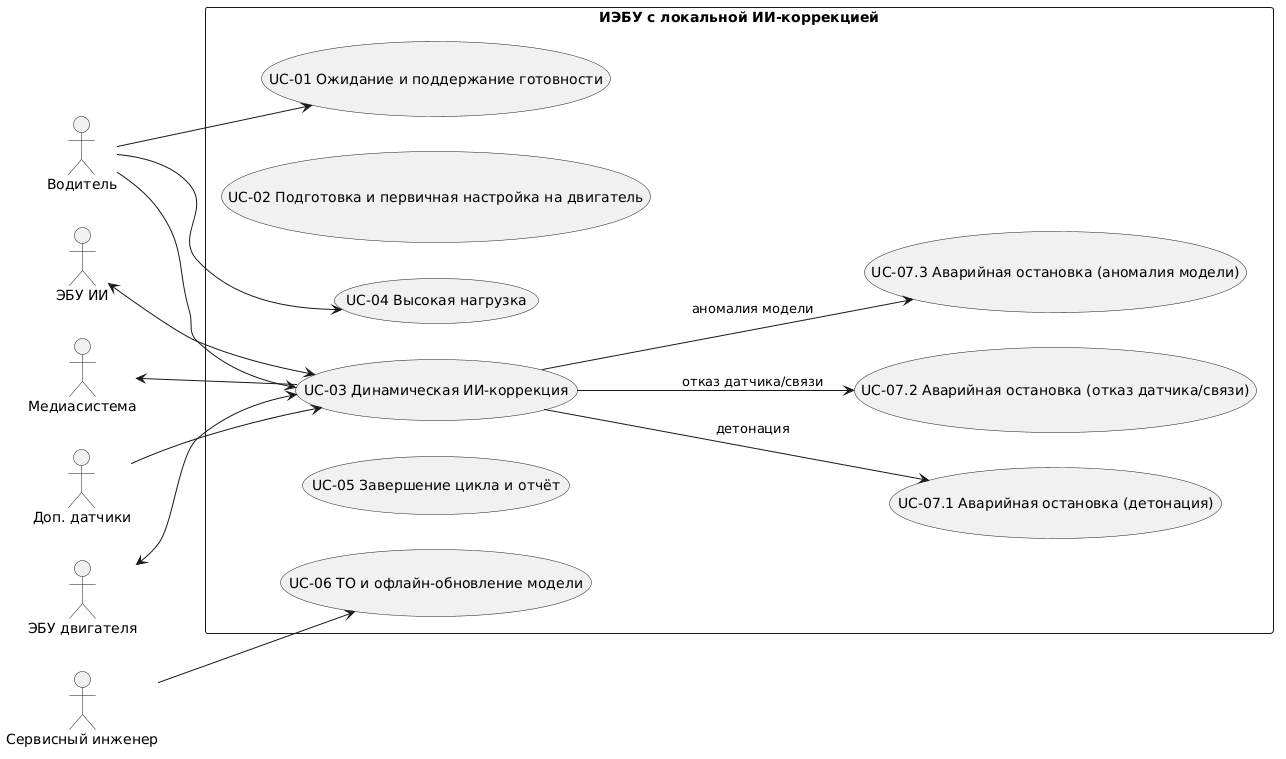
\includegraphics[width=1\linewidth]{pic/ZLJ1QXDH5Ds}
						\caption{Диаграмма Use Case}
						\label{fig:zlj1qxdh5ds}
					\end{figure}
					
				\subsection{Основные сценарии}
					{\fontsize{9}{11}\selectfont
						\begin{xltabular}{\textwidth}{|c|L|L|L|L|L|L|L|}
						\caption{Основные сценарии использования}\label{tab:usecases-main}\\
						\hline
						\textbf{ID} & \textbf{Режим} & \textbf{Use Case} & \textbf{Основной актор} & \textbf{Краткое описание} & \textbf{Предусловия} & \textbf{Основной поток} & \textbf{Постусловия} \\
						\hline
						\endfirsthead
						\hline
						\textbf{ID} & \textbf{Режим} & \textbf{Use Case} & \textbf{Основной актор} & \textbf{Краткое описание} & \textbf{Предусловия} & \textbf{Основной поток} & \textbf{Постусловия} \\
						\hline
						\endhead
						\hline
						\endfoot
						\hline
						\endlastfoot
						UC-01 & Ожидание (S2) & Поддержание режима ожидания & ЭБУ ИИ, ЭБУ двигателя & Поддержание фоновой готовности; связь между блоками активна & Система в S2; связь CAN/Ethernet установлена & 1. ЭБУ ИИ периодически отправляет сигналы. 2. ЭБУ двигателя подтверждает приём. 3. При отклонении — переход в S3 (диагностика) & Состояние S2 сохраняется \\
						\hline
						UC-02 & Подготовка (S3–S4) & Подготовка и первичная настройка на двигатель & ЭБУ ИИ & Построение начальной модели конкретного двигателя при первом включении & Система в S3; датчики исправны; модель загружена & 1. ЭБУ ИИ читает показания датчиков с ЭБУ двигателя. 2. Строит начальную модель (идентификация параметров). 3. Формирует базовые поправки. 4. Регистрирует модель и версию в аудит-трейсе. 5. Переход в S5 & Модель двигателя построена; базовые поправки сформированы \\
						\hline
						UC-03 & Нормальная эксплуатация (S5) & Динамическая ИИ-коррекция & ЭБУ ИИ, ЭБУ двигателя & Динамическая коррекция коэффициентов по ходу движения & Система в S5; модель двигателя построена & 1. ЭБУ ИИ читает датчики (включая дополнительные). 2. Анализирует данные, формирует поправки. 3. ЭБУ двигателя валидирует поправки в безопасных пределах. 4. Применяет воздействия. 5. Контроль результата (лямбда, детонация, расход). 6. Логирование & Коэффициенты обновлены; лог сохранён \\
						\hline
						UC-04 & Высокая нагрузка (S6) & Коррекция при высокой нагрузке & ЭБУ ИИ, ЭБУ двигателя & Приоритет мощности; коррекция УОЗ/наддува с ограничением по детонации & Система в S5; детекция высокой нагрузки & 1. Детекция высокой нагрузки. 2. Коррекция УОЗ/наддува с ограничением по детонации. 3. Контроль. 4. При опасной детонации — UC-07.1 & Коэффициенты обновлены; детонация в пределах \\
						\hline
						UC-05 & Завершение (S9–S10) & Завершение цикла и отчёт & ЭБУ ИИ, ЭБУ двигателя & Завершение цикла, формирование отчёта, передача в OBD-II/медиасистему & Завершение движения; зажигание выключено & 1. Сброс временных поправок. 2. Генерация лога коррекций. 3. Формирование аудит-трейса. 4. Передача в OBD-II/медиасистему. 5. Переход в S11 & Отчёт сформирован; система в S11 \\
						\hline
					\end{xltabular}}
					
				\subsection{Сервисные сценарии}
					{\fontsize{9}{11}\selectfont
						\begin{xltabular}{\textwidth}{|c|L|L|L|L|L|L|L|}
						\caption{Сервисные сценарии использования}\label{tab:usecases-service}\\
						\hline
						\textbf{ID} & \textbf{Режим} & \textbf{Use Case} & \textbf{Основной актор} & \textbf{Краткое описание} & \textbf{Предусловия} & \textbf{Основной поток} & \textbf{Постусловия} \\
						\hline
						\endfirsthead
						\hline
						\textbf{ID} & \textbf{Режим} & \textbf{Use Case} & \textbf{Основной актор} & \textbf{Краткое описание} & \textbf{Предусловия} & \textbf{Основной поток} & \textbf{Постусловия} \\
						\hline
						\endhead
						\hline
						\endfoot
						\hline
						\endlastfoot
						UC-06.1 & ТО (S12) & Проведение ТО & Сервисный инженер & Регламентное/аварийное ТО & Система в S12; авторизация пройдена & 1. Ввод пароля/RFID. 2. Диагностика. 3. Устранение неполадок. 4. Подтверждение исправности. 5. Переход в S2 & Система исправна; S2 \\
						\hline
						UC-06.2 & Обновление (S13) & Офлайн-обновление модели & Сервисный инженер & Загрузка новой нейросетевой модели через защищённый интерфейс & Система в S13; пакет получен & 1. Загрузка пакета. 2. Проверка подписи и целостности. 3. Активация модели. 4. При ошибке — откат. 5. Переход в S2 & Новая модель активна; S2 \\
						\hline
					\end{xltabular}}
					
				\subsection{Аварийные сценарии}
					{\fontsize{9}{11}\selectfont
						\begin{xltabular}{\textwidth}{|L|L|L|L|L|L|L|L|}
						\caption{Аварийные сценарии использования}\label{tab:usecases-emergency}\\
						\hline
						\textbf{ID} & \textbf{Режим} & \textbf{Use Case} & \textbf{Основной актор} & \textbf{Краткое описание} & \textbf{Пред- условия} & \textbf{Основной поток} & \textbf{Постусловия} \\
						\hline
						\endfirsthead
						\hline
						\textbf{ID} & \textbf{Режим} & \textbf{Use Case} & \textbf{Основной актор} & \textbf{Краткое описание} & \textbf{Пред- условия} & \textbf{Основной поток} & \textbf{Постусловия} \\
						\hline
						\endhead
						\hline
						\endfoot
						\hline
						\endlastfoot
						UC-07.1 & Авария (S8) & Аварийная остановка при детонации & ЭБУ двигателя & Безопасное завершение при опасной детонации & Детонация выше порога & 1. Детекция опасной детонации. 2. Отключение ИИ-коррекции. 3. Переход на базовые калибровки. 4. Формирование DTC. 5. Уведомление водителя. 6. Переход в S8 & Система в S8; DTC сформирован \\
						\hline
						UC-07.2 & Авария (S8) & Аварийная остановка при отказе датчика/связи & ЭБУ двигателя & Безопасное завершение при отказе датчика или потере связи между блоками & Отказ датчика/потеря связи & 1. Диагностика обнаруживает отказ. 2. Отключение ИИ-коррекции. 3. Переход на базовые калибровки. 4. Формирование DTC. 5. Уведомление водителя. 6. Переход в S8 & Система в S8; DTC сформирован \\
						\hline
						UC-07.3 & Авария (S8) & Аварийная остановка при аномалии модели & ЭБУ ИИ & Безопасное завершение при обнаружении аномалии в модели & Аномалия в модели (выход за пределы) & 1. Детекция аномалии. 2. Отключение ИИ-коррекции. 3. Переход на базовые калибровки. 4. Формирование DTC. 5. Уведомление водителя. 6. Переход в S8 & Система в S8; DTC сформирован \\
						\hline
					\end{xltabular}}
					
				\subsection{Диаграмма последовательности (UC-03 «Динамическая ИИ-коррекция»)}
				
					\begin{figure}[H]
						\centering
						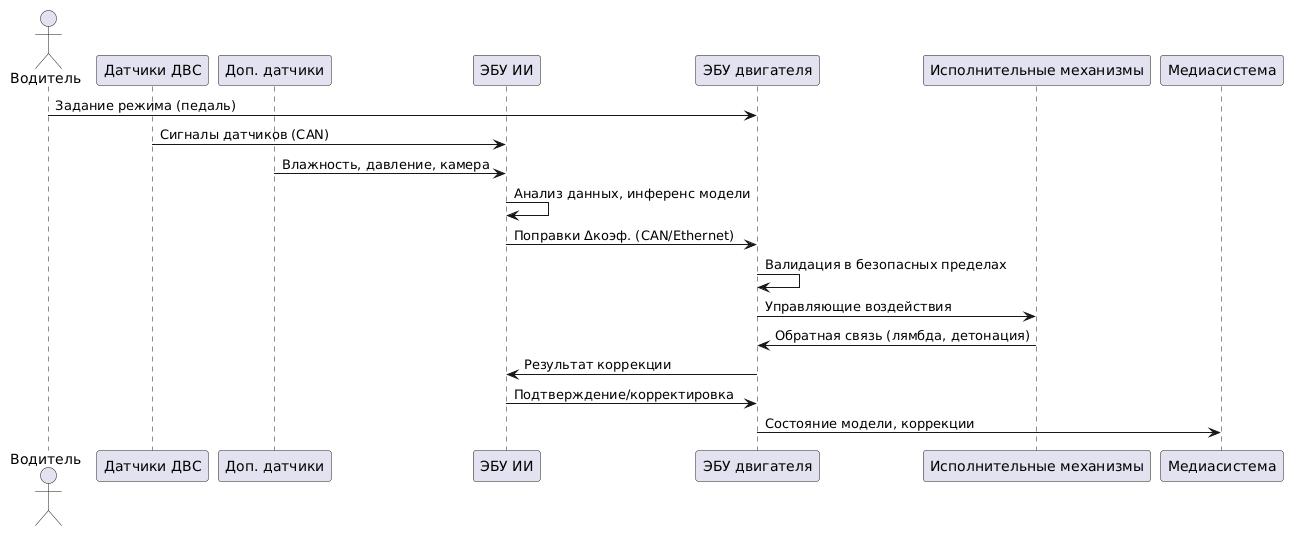
\includegraphics[width=1\linewidth]{pic/RLFDJXfX5DtFKtnnXOa.png}
						\caption{Диаграмма последовательности}
						\label{fig:rlfdjx}
					\end{figure}
					
					
					Описание: ЭБУ ИИ читает датчики (включая дополнительные), анализирует данные и формирует поправки; ЭБУ двигателя валидирует их в безопасных пределах и применяет к исполнительным механизмам; обратная связь по лямбде/детонации возвращается в ЭБУ ИИ; состояние модели и коррекции выводятся на медиасистему. ИИ не управляет ДВС напрямую.
					
				\subsection{Диаграмма переходов между сценариями}
				
					\begin{figure}[H]
						\centering
						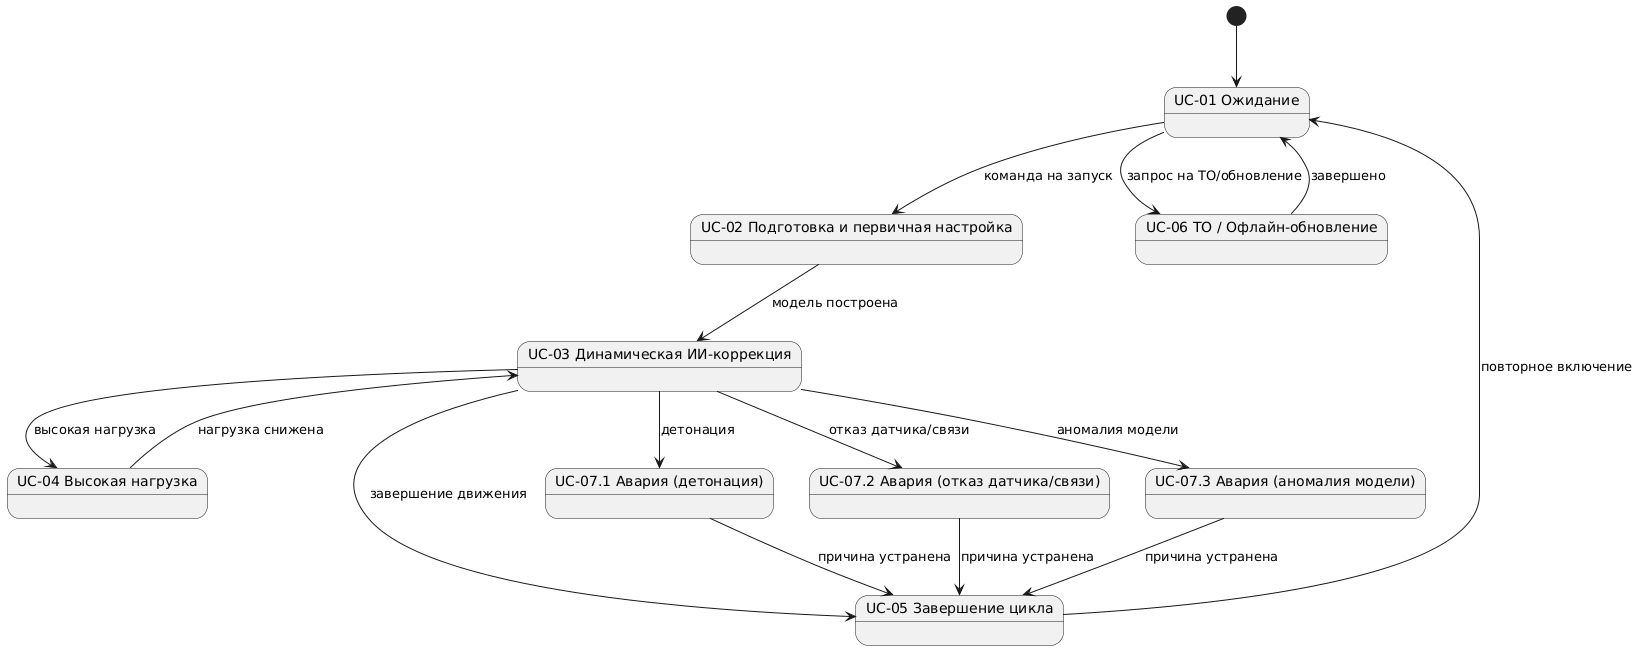
\includegraphics[width=1\linewidth]{pic/sZLN4dn.png}
						\caption{Диаграмма переходов между сценариями}
						\label{fig:szln}
					\end{figure}
				
				\subsection{Связь сценариев с режимами и функциями}
					\begin{xltabular}{\textwidth}{|L|L|L|L|}
						\caption{Связь сценариев с режимами и функциями}\label{tab:uc-modes-functions}\\
						\hline
						\textbf{Use Case} & \textbf{Режим (S)} & \textbf{Функции (C)} & \textbf{Цели (G)} \\
						\hline
						\endfirsthead
						\hline
						\textbf{Use Case} & \textbf{Режим (S)} & \textbf{Функции (C)} & \textbf{Цели (G)} \\
						\hline
						\endhead
						\hline
						\endfoot
						\hline
						\endlastfoot
						UC-01 & S2 & C.01, C.06 & G.02 \\
						\hline
						UC-02 & S3–S4 & C.01, C.02, C.03 & G.01, G.04 \\
						\hline
						UC-03 & S5, S7 & C.01–C.05 & G.01, G.02, G.03, G.04, G.05 \\
						\hline
						UC-04 & S6 & C.03, C.04 & G.02 \\
						\hline
						UC-05 & S9–S10 & C.06 & G.03, G.05 \\
						\hline
						UC-06.1 & S12 & C.06 & G.02, G.03 \\
						\hline
						UC-06.2 & S13 & C.06 & G.04, G.05 \\
						\hline
						UC-07.1 & S8 & C.04, C.06 & G.02 \\
						\hline
						UC-07.2 & S8 & C.04, C.06 & G.02 \\
						\hline
						UC-07.3 & S8 & C.04, C.06 & G.02 \\
						\hline
					\end{xltabular}
					
				\section{Трассировка сценариев взаимодействия с шагами деятельности в надсистеме}
				
				\subsection{Общие положения}
				
				Трассировка сценариев к деятельности надсистемы обеспечивает прослеживаемость от бизнес-процессов до технических функций системы ИЭБУ. Таблица~\ref{tab:uc-trace} демонстрирует, как автоматизация преобразует существующие процессы управления ДВС, выявляет зоны замены ручных операций и оптимизации, а также показывает, какие шаги деятельности надсистемы поддерживаются или заменяются каждым сценарием взаимодействия.
				
				\textbf{Надсистема:} процесс управления ДВС в составе автомобиля.
				
				\textbf{Основной процесс надсистемы:} «Обеспечить эффективную, экологичную и безопасную работу ДВС в реальных условиях эксплуатации».
				
				\textbf{Шаги деятельности в надсистеме (AS-IS / TO-BE):}
				\begin{enumerate}
					\item Сбор данных — чтение датчиков (ДМРВ/ДАД, лямбда, ДПКВ, ДПРВ, детонация, t° ОЖ/воздуха, давление топлива).
					\item Оценка состояния — расчёт режима (нагрузка/обороты), детекция аномалий.
					\item Коррекция калибровок — формирование поправок коэффициентов (топливо, УОЗ, наддув, EGR).
					\item Применение воздействий — формирование сигналов на исполнительные механизмы.
					\item Контроль результата — обратная связь по лямбде, детонации, расходу.
					\item Диагностика и логирование — DTC, логи, аудит-трейс.
					\item Обслуживание и обновление — ТО, офлайн-обновление модели.
				\end{enumerate}
				
				\subsection{Трассировка сценариев с шагами деятельности в надсистеме}
				
				{\fontsize{9}{11}\selectfont
					\begin{xltabular}{\textwidth}{|c|L|L|L|}
					\caption{Трассировка сценариев взаимодействия с шагами деятельности в надсистеме}\label{tab:uc-trace}\\
					\hline
					\textbf{Use Case} & \textbf{Наименование} & \textbf{Шаги деятельности в надсистеме (AS-IS), поддерживаемые/заменяемые UC} & \textbf{Комментарий} \\
					\hline
					\endfirsthead
					\hline
					\textbf{Use Case} & \textbf{Наименование} & \textbf{Шаги деятельности в надсистеме (AS-IS), поддерживаемые/заменяемые UC} & \textbf{Комментарий} \\
					\hline
					\endhead
					\hline
					\endfoot
					\hline
					\endlastfoot
					UC-01 & Поддержание режима ожидания & — & Не имеет прямого аналога в ручном процессе. Поддерживает общую готовность системы между циклами — аналогично фоновому контролю. Косвенно поддерживает все этапы. \\
					\hline
					UC-02 & Подготовка и первичная настройка на двигатель & 1. Сбор данных (частично) & Заменяет стендовые калибровки: ЭБУ ИИ строит начальную модель конкретного двигателя по данным датчиков, формирует базовые поправки. Ранее выполнялось вручную на стенде. \\
					\hline
					UC-03 & Динамическая ИИ-коррекция & 1. Сбор данных; 2. Оценка состояния; 3. Коррекция калибровок; 4. Применение воздействий; 5. Контроль результата & Прямая автоматизация этапов 1–5 в реальном времени по ходу движения. Заменяет статические таблицы на адаптивный контур. \\
					\hline
					UC-04 & Коррекция при высокой нагрузке & 3. Коррекция калибровок; 4. Применение воздействий; 5. Контроль результата & Адаптация под высокую нагрузку с приоритетом мощности и ограничением по детонации. \\
					\hline
					UC-05 & Завершение цикла и отчёт & 6. Диагностика и логирование & Автоматизирует контроль (через датчики + анализ) и генерацию отчёта (вместо бумажного/устного доклада). \\
					\hline
					UC-06.1 & Проведение ТО & 7. Обслуживание и обновление & Регламентное/аварийное ТО; аналог человеческого ТО оборудования между сменами. \\
					\hline
					UC-06.2 & Офлайн-обновление модели & 7. Обслуживание и обновление & Обновление нейросетевой модели через защищённый сервисный интерфейс (без интернета/облака/OTA). \\
					\hline
					UC-07.1 & Аварийная остановка при детонации & 4. Применение воздействий (fail-safe); 6. Диагностика и логирование & Обеспечивает безопасное завершение при опасной детонации: отключение ИИ-коррекции, переход на базовые калибровки, DTC. \\
					\hline
					UC-07.2 & Аварийная остановка при отказе датчика/связи & 4. Применение воздействий (fail-safe); 6. Диагностика и логирование & Безопасное завершение при отказе датчика или потере связи между блоками. \\
					\hline
					UC-07.3 & Аварийная остановка при аномалии модели & 4. Применение воздействий (fail-safe); 6. Диагностика и логирование & Безопасное завершение при обнаружении аномалии в модели (выход за пределы). \\
					\hline
				\end{xltabular}}
				
				\subsection{Детализация трассировки по шагам деятельности}
				
				\subsubsection{Шаг «Сбор данных»}
				
				{\fontsize{9}{11}\selectfont
					\begin{xltabular}{\textwidth}{|L|L|L|L|}
					\caption{Детализация трассировки шага «Сбор данных»}\label{tab:trace-collect}\\
					\hline
					\textbf{Аспект} & \textbf{AS-IS} & \textbf{TO-BE (с ИЭБУ)} & \textbf{Сценарий} \\
					\hline
					\endfirsthead
					\hline
					\textbf{Аспект} & \textbf{AS-IS} & \textbf{TO-BE (с ИЭБУ)} & \textbf{Сценарий} \\
					\hline
					\endhead
					\hline
					\endfoot
					\hline
					\endlastfoot
					Источник данных & Датчики ДВС & Датчики ДВС + дополнительные (влажность, давление, камера) & UC-03 \\
					\hline
					Частота & По циклу ЭБУ & \(\geq 100\) Гц, непрерывно & UC-03 \\
					\hline
					Валидация & В ЭБУ двигателя & В ЭБУ ИИ + ЭБУ двигателя & UC-03 \\
					\hline
					Передача & Внутри ЭБУ & CAN/Ethernet между блоками & UC-03 \\
					\hline
				\end{xltabular}}
				
				\subsubsection{Шаг «Оценка состояния»}
				
				{\fontsize{9}{11}\selectfont
					\begin{xltabular}{\textwidth}{|L|L|L|L|}
					\caption{Детализация трассировки шага «Оценка состояния»}\label{tab:trace-estimate}\\
					\hline
					\textbf{Аспект} & \textbf{AS-IS} & \textbf{TO-BE (с ИЭБУ)} & \textbf{Сценарий} \\
					\hline
					\endfirsthead
					\hline
					\textbf{Аспект} & \textbf{AS-IS} & \textbf{TO-BE (с ИЭБУ)} & \textbf{Сценарий} \\
					\hline
					\endhead
					\hline
					\endfoot
					\hline
					\endlastfoot
					Расчёт режима & В ЭБУ двигателя & В ЭБУ ИИ (модель) + ЭБУ двигателя & UC-03 \\
					\hline
					Детекция аномалий & Пороговая, статическая & Адаптивная, на основе модели & UC-03, UC-07.x \\
					\hline
					Учёт износа/топлива/климата & Нет & Да (модель обновляется) & UC-03 \\
					\hline
				\end{xltabular}}
				
				\subsubsection{Шаг «Коррекция калибровок»}
				
				{\fontsize{9}{11}\selectfont
					\begin{xltabular}{\textwidth}{|L|L|L|L|}
					\caption{Детализация трассировки шага «Коррекция калибровок»}\label{tab:trace-correction}\\
					\hline
					\textbf{Аспект} & \textbf{AS-IS} & \textbf{TO-BE (с ИЭБУ)} & \textbf{Сценарий} \\
					\hline
					\endfirsthead
					\hline
					\textbf{Аспект} & \textbf{AS-IS} & \textbf{TO-BE (с ИЭБУ)} & \textbf{Сценарий} \\
					\hline
					\endhead
					\hline
					\endfoot
					\hline
					\endlastfoot
					Источник поправок & Статические таблицы & Локальная ИИ-модель & UC-02, UC-03, UC-04 \\
					\hline
					Валидация & — & В ЭБУ двигателя (безопасные пределы) & UC-03, UC-04 \\
					\hline
					Логирование & — & Аудит-трейс & UC-03, UC-05 \\
					\hline
				\end{xltabular}}
				
				\subsubsection{Шаг «Применение воздействий»}
				
				{\fontsize{9}{11}\selectfont
					\begin{xltabular}{\textwidth}{|L|L|L|L|}
					\caption{Детализация трассировки шага «Применение воздействий»}\label{tab:trace-apply}\\
					\hline
					\textbf{Аспект} & \textbf{AS-IS} & \textbf{TO-BE (с ИЭБУ)} & \textbf{Сценарий} \\
					\hline
					\endfirsthead
					\hline
					\textbf{Аспект} & \textbf{AS-IS} & \textbf{TO-BE (с ИЭБУ)} & \textbf{Сценарий} \\
					\hline
					\endhead
					\hline
					\endfoot
					\hline
					\endlastfoot
					Управление & ЭБУ двигателя & ЭБУ двигателя (ИИ не управляет напрямую) & UC-03, UC-04 \\
					\hline
					Fail-safe & Пороговый & Адаптивный + откат & UC-07.x \\
					\hline
					Ограничения & Статические & Динамические (по модели) & UC-04 \\
					\hline
				\end{xltabular}}
				
				\subsubsection{Шаг «Контроль результата»}
				
				{\fontsize{9}{11}\selectfont
					\begin{xltabular}{\textwidth}{|L|L|L|L|}
					\caption{Детализация трассировки шага «Контроль результата»}\label{tab:trace-control}\\
					\hline
					\textbf{Аспект} & \textbf{AS-IS} & \textbf{TO-BE (с ИЭБУ)} & \textbf{Сценарий} \\
					\hline
					\endfirsthead
					\hline
					\textbf{Аспект} & \textbf{AS-IS} & \textbf{TO-BE (с ИЭБУ)} & \textbf{Сценарий} \\
					\hline
					\endhead
					\hline
					\endfoot
					\hline
					\endlastfoot
					Обратная связь & Лямбда, детонация & Лямбда, детонация, расход + модель & UC-03 \\
					\hline
					Оценка эффективности & Нет & Да (сравнение с ожиданием) & UC-03 \\
					\hline
					Решение о продолжении/откате & Нет & Да & UC-03, UC-07.x \\
					\hline
				\end{xltabular}}
				
				\subsubsection{Шаг «Диагностика и логирование»}
				
				{\fontsize{9}{11}\selectfont
					\begin{xltabular}{\textwidth}{|L|L|L|L|}
					\caption{Детализация трассировки шага «Диагностика и логирование»}\label{tab:trace-diagnostics}\\
					\hline
					\textbf{Аспект} & \textbf{AS-IS} & \textbf{TO-BE (с ИЭБУ)} & \textbf{Сценарий} \\
					\hline
					\endfirsthead
					\hline
					\textbf{Аспект} & \textbf{AS-IS} & \textbf{TO-BE (с ИЭБУ)} & \textbf{Сценарий} \\
					\hline
					\endhead
					\hline
					\endfoot
					\hline
					\endlastfoot
					DTC & Пороговые & Адаптивные & UC-05, UC-07.x \\
					\hline
					Логи & Минимальные & Полный аудит-трейс & UC-05 \\
					\hline
					Передача & OBD-II & OBD-II + медиасистема & UC-05 \\
					\hline
				\end{xltabular}}
				
				\subsubsection{Шаг «Обслуживание и обновление»}
				
				{\fontsize{9}{11}\selectfont
					\begin{xltabular}{\textwidth}{|L|L|L|L|}
					\caption{Детализация трассировки шага «Обслуживание и обновление»}\label{tab:trace-maintenance}\\
					\hline
					\textbf{Аспект} & \textbf{AS-IS} & \textbf{TO-BE (с ИЭБУ)} & \textbf{Сценарий} \\
					\hline
					\endfirsthead
					\hline
					\textbf{Аспект} & \textbf{AS-IS} & \textbf{TO-BE (с ИЭБУ)} & \textbf{Сценарий} \\
					\hline
					\endhead
					\hline
					\endfoot
					\hline
					\endlastfoot
					ТО & Регламентное & Регламентное + аварийное & UC-06.1 \\
					\hline
					Обновление & Прошивка ЭБУ & Офлайн-обновление модели через защищённый интерфейс & UC-06.2 \\
					\hline
					Безопасность & — & Подпись, анти-tamper & UC-06.2 \\
					\hline
				\end{xltabular}}
				
				\subsection{Сводная матрица «Сценарий \(\times\) Шаг деятельности»}
				
				{\fontsize{9}{11}\selectfont
					\begin{xltabular}{\textwidth}{|c|L|L|L|L|L|L|L|}
					\caption{Матрица покрытия шагов деятельности сценариями}\label{tab:coverage}\\
					\hline
					\textbf{Сценарий} & \textbf{1. Сбор данных} & \textbf{2. Оценка состояния} & \textbf{3. Коррекция калибровок} & \textbf{4. Применение воздействий} & \textbf{5. Контроль результата} & \textbf{6. Диагностика и логирование} & \textbf{7. Обслуживание и обновление} \\
					\hline
					\endfirsthead
					\hline
					\textbf{Сценарий} & \textbf{1. Сбор данных} & \textbf{2. Оценка состояния} & \textbf{3. Коррекция калибровок} & \textbf{4. Применение воздействий} & \textbf{5. Контроль результата} & \textbf{6. Диагностика и логирование} & \textbf{7. Обслуживание и обновление} \\
					\hline
					\endhead
					\hline
					\endfoot
					\hline
					\endlastfoot
					UC-01 & + & — & — & — & — & + & — \\
					\hline
					UC-02 & + & + & + & — & — & + & — \\
					\hline
					UC-03 & + & + & + & + & + & + & — \\
					\hline
					UC-04 & + & + & + & + & + & + & — \\
					\hline
					UC-05 & — & — & — & — & + & + & — \\
					\hline
					UC-06.1 & — & — & — & — & — & + & + \\
					\hline
					UC-06.2 & — & — & — & — & — & + & + \\
					\hline
					UC-07.1 & — & + & — & + & — & + & — \\
					\hline
					UC-07.2 & — & + & — & + & — & + & — \\
					\hline
					UC-07.3 & — & + & — & + & — & + & — \\
					\hline
				\end{xltabular}}
				
				\textbf{Обозначения:} «+» — сценарий покрывает шаг; «—» — не покрывает.
				
				\subsection{Ключевые выводы по трассировке}
				
				\begin{enumerate}
					\item \textbf{UC-03 (Динамическая ИИ-коррекция)} — центральный сценарий, покрывающий шаги 1–6 деятельности надсистемы. Именно он реализует ключевое отличие TO-BE от AS-IS: динамическую коррекцию коэффициентов по ходу движения.
					\item \textbf{UC-02 (Первичная настройка)} — заменяет стендовые калибровки: модель строится автоматически по данным датчиков, что сокращает время настройки на конкретный двигатель.
					\item \textbf{UC-07.x (Аварийные сценарии)} — обеспечивают безопасность при аномалиях, покрывая шаги 2 (детекция), 4 (fail-safe) и 6 (DTC). Это соответствует требованию ISO 26262/21448.
					\item \textbf{UC-06.x (Сервисные сценарии)} — покрывают шаг 7 (обслуживание и обновление), обеспечивая maintainability и обновляемость модели \textbf{без интернета/облака/OTA}.
					\item \textbf{Полное покрытие:} все 7 шагов деятельности надсистемы покрыты хотя бы одним сценарием, что подтверждает полноту набора Use Case.
					\item \textbf{Принцип безопасности:} ИИ \textbf{не управляет ДВС напрямую} — во всех сценариях применение воздействий (шаг 4) выполняется ЭБУ двигателя с валидацией поправок и fail-safe.
				\end{enumerate}
				
				
			\section{Описание функций системы в соответствии с установленными сценариями}
			
				\subsection{Общие положения}
				
					Функциональная модель системы ИЭБУ разработана на основе сценариев взаимодействия (п.~6) и представляет собой логическую декомпозицию возможностей системы на элементарные функции. Каждая функция определена как преобразование входных воздействий в выходные результаты при соблюдении заданных ограничений. Такой подход обеспечивает полноту охвата требований и возможность верификации выполнения каждой функции.
					
					\textbf{Принципы выделения функций:}
					\begin{itemize}
						\item \textbf{Следование сценариям:} каждому основному сценарию взаимодействия соответствует набор функций, реализующих конкретные операции.
						\item \textbf{Независимость:} функции спроектированы для минимизации взаимных зависимостей, что повышает надёжность и упрощает модификацию.
						\item \textbf{Измеримость:} для каждой функции определены количественные параметры эффективности (время выполнения, точность, надёжность).
						\item \textbf{Связь с целями:} каждая функция трассируется к конкретным целям системы и заинтересованным сторонам.
					\end{itemize}
					
					\textbf{Функции системы сгруппированы по функциональным областям:}
					\begin{itemize}
						\item \textbf{Функции сбора и оценки} (F.01–F.03): обеспечивают достоверность входных данных и оценку состояния двигателя.
						\item \textbf{Функции динамической коррекции} (F.04–F.06): реализуют основное назначение системы — динамическую ИИ-коррекцию коэффициентов.
						\item \textbf{Функции применения и контроля} (F.07–F.08): обеспечивают безопасное применение воздействий и оценку результата.
						\item \textbf{Функции диагностики и поддержки} (F.09–F.11): поддерживают работоспособность, прослеживаемость и обновляемость системы.
					\end{itemize}
					
					\subsection{Таблица функций системы}
					
					\begin{xltabular}{\textwidth}{|c|L|L|L|}
						\caption{Функции системы в соответствии с установленными сценариями}\label{tab:functions}\\
						\hline
						\textbf{№} & \textbf{Наименование функции} & \textbf{Трассировка} & \textbf{Описание (Вход \(\to\) Операция \(\to\) Выход)} \\
						\hline
						\endfirsthead
						\hline
						\textbf{№} & \textbf{Наименование функции} & \textbf{Трассировка} & \textbf{Описание (Вход \(\to\) Операция \(\to\) Выход)} \\
						\hline
						\endhead
						\hline
						\endfoot
						\hline
						\endlastfoot
						F.01 & Приём и валидация сигналов датчиков & UC-01, UC-02, UC-03 \(\to\) C.01 \(\to\) G.01 & Сигналы датчиков (CAN/аналог) \(\to\) проверка диапазонов, достоверности, синхронизации \(\to\) валидированные данные (частота \(\geq 100\) Гц) \\
						\hline
						F.02 & Оценка режима работы двигателя & UC-03 \(\to\) C.02 \(\to\) G.01 & Валидированные данные \(\to\) расчёт нагрузки/оборотов, идентификация режима \(\to\) текущий режим \\
						\hline
						F.03 & Детекция аномалий & UC-03, UC-07.x \(\to\) C.02 \(\to\) G.02 & Данные + модель \(\to\) детекция детонации, пропусков, обеднения/обогащения \(\to\) флаги аномалий \\
						\hline
						F.04 & Построение/обновление модели двигателя & UC-02 \(\to\) C.03 \(\to\) G.01, G.04 & Данные датчиков (включая дополнительные) \(\to\) идентификация параметров, обучение/обновление модели \(\to\) модель конкретного двигателя \\
						\hline
						F.05 & Формирование поправок коэффициентов (ИИ-инференс) & UC-03, UC-04 \(\to\) C.03 \(\to\) G.01, G.02 & Признаки + модель \(\to\) инференс нейросети \(\to\) поправки \(\Delta\)коэф. (топливо, УОЗ, наддув, EGR) \\
						\hline
						F.06 & Валидация поправок в безопасных пределах & UC-03, UC-04 \(\to\) C.04 \(\to\) G.02 & Поправки \(\to\) проверка пределов (детонация, ресурс, экология) \(\to\) безопасные поправки (или откат) \\
						\hline
						F.07 & Применение управляющих воздействий & UC-03, UC-04 \(\to\) C.04 \(\to\) G.01, G.02 & Безопасные поправки \(\to\) формирование PWM/дискретных сигналов \(\to\) воздействия на исполнительные механизмы \\
						\hline
						F.08 & Контроль результата коррекции & UC-03 \(\to\) C.05 \(\to\) G.01, G.02, G.05 & Обратная связь (лямбда, детонация, расход) \(\to\) сравнение с ожиданием \(\to\) оценка эффективности, решение о продолжении/откате \\
						\hline
						F.09 & Fail-safe и откат & UC-07.x \(\to\) C.04, C.05 \(\to\) G.02 & Аномалия/отказ \(\to\) отключение ИИ-коррекции, переход на базовые калибровки \(\to\) безопасное состояние, DTC \\
						\hline
						F.10 & Диагностика, логирование и аудит-трейс & UC-05, UC-07.x \(\to\) C.06 \(\to\) G.03, G.05 & События/коррекции \(\to\) формирование DTC, логов, аудит-трейса \(\to\) данные для OBD-II/медиасистемы \\
						\hline
						F.11 & Офлайн-обновление модели & UC-06.2 \(\to\) C.06 \(\to\) G.04, G.05 & Пакет обновления \(\to\) проверка подписи/целостности, активация/откат \(\to\) новая модель (или предыдущая) \\
						\hline
					\end{xltabular}
					
					\subsection{Детализация функций по сценариям}
					
					\subsubsection{UC-01 «Поддержание режима ожидания»}
					
					\begin{xltabular}{\textwidth}{|c|L|L|}
						\caption{Функции сценария UC-01}\label{tab:func-uc01}\\
						\hline
						\textbf{Функция} & \textbf{Описание} & \textbf{Параметры} \\
						\hline
						\endfirsthead
						\hline
						\textbf{Функция} & \textbf{Описание} & \textbf{Параметры} \\
						\hline
						\endhead
						\hline
						\endfoot
						\hline
						\endlastfoot
						F.01 & Периодический опрос датчиков и валидация & Частота \(\geq 100\) Гц; задержка \(\leq 1\) мс \\
						\hline
						F.10 & Фоновая диагностика, логирование состояния & Периодичность логирования \(\leq 1\) с \\
						\hline
					\end{xltabular}
					
					\subsubsection{UC-02 «Подготовка и первичная настройка на двигатель»}
					
					\begin{xltabular}{\textwidth}{|c|L|L|}
						\caption{Функции сценария UC-02}\label{tab:func-uc02}\\
						\hline
						\textbf{Функция} & \textbf{Описание} & \textbf{Параметры} \\
						\hline
						\endfirsthead
						\hline
						\textbf{Функция} & \textbf{Описание} & \textbf{Параметры} \\
						\hline
						\endhead
						\hline
						\endfoot
						\hline
						\endlastfoot
						F.01 & Сбор данных с датчиков (включая дополнительные) & Частота \(\geq 100\) Гц \\
						\hline
						F.02 & Оценка режима & Задержка \(\leq 5\) мс \\
						\hline
						F.04 & Построение начальной модели двигателя & Время построения \(\leq 10\) мин \\
						\hline
						F.10 & Регистрация модели и версии в аудит-трейсе & Полнота 100\% \\
						\hline
					\end{xltabular}
					
					\subsubsection{UC-03 «Динамическая ИИ-коррекция»}
					
					\begin{xltabular}{\textwidth}{|c|L|L|}
						\caption{Функции сценария UC-03}\label{tab:func-uc03}\\
						\hline
						\textbf{Функция} & \textbf{Описание} & \textbf{Параметры} \\
						\hline
						\endfirsthead
						\hline
						\textbf{Функция} & \textbf{Описание} & \textbf{Параметры} \\
						\hline
						\endhead
						\hline
						\endfoot
						\hline
						\endlastfoot
						F.01 & Сбор и валидация сигналов датчиков & Частота \(\geq 100\) Гц; задержка \(\leq 10\) мс \\
						\hline
						F.02 & Оценка режима & Задержка \(\leq 5\) мс \\
						\hline
						F.03 & Детекция аномалий & Задержка \(\leq 5\) мс; ложное срабатывание \(\leq 0{,}5\%\) \\
						\hline
						F.05 & ИИ-инференс поправок & Задержка \(\leq 5\) мс; точность \(\leq 2\%\) \\
						\hline
						F.06 & Валидация поправок & \(100\%\) поправок проверены \\
						\hline
						F.07 & Применение воздействий & Задержка \(\leq 10\) мс \\
						\hline
						F.08 & Контроль результата & Оценка каждого цикла \\
						\hline
						F.10 & Логирование и аудит-трейс & \(100\%\) коррекций залогированы \\
						\hline
					\end{xltabular}
					
					\subsubsection{UC-04 «Коррекция при высокой нагрузке»}
					
					\begin{xltabular}{\textwidth}{|c|L|L|}
						\caption{Функции сценария UC-04}\label{tab:func-uc04}\\
						\hline
						\textbf{Функция} & \textbf{Описание} & \textbf{Параметры} \\
						\hline
						\endfirsthead
						\hline
						\textbf{Функция} & \textbf{Описание} & \textbf{Параметры} \\
						\hline
						\endhead
						\hline
						\endfoot
						\hline
						\endlastfoot
						F.02 & Детекция высокой нагрузки & Задержка \(\leq 5\) мс \\
						\hline
						F.05 & Коррекция УОЗ/наддува с ограничением по детонации & Точность \(\leq 2\%\) \\
						\hline
						F.06 & Валидация с приоритетом безопасности & \(100\%\) \\
						\hline
						F.07 & Применение воздействий & Задержка \(\leq 10\) мс \\
						\hline
						F.09 & Переход в UC-07.1 при опасной детонации & Время реакции \(\leq 200\) мс \\
						\hline
					\end{xltabular}
					
					\subsubsection{UC-05 «Завершение цикла и отчёт»}
					
					\begin{xltabular}{\textwidth}{|c|L|L|}
						\caption{Функции сценария UC-05}\label{tab:func-uc05}\\
						\hline
						\textbf{Функция} & \textbf{Описание} & \textbf{Параметры} \\
						\hline
						\endfirsthead
						\hline
						\textbf{Функция} & \textbf{Описание} & \textbf{Параметры} \\
						\hline
						\endhead
						\hline
						\endfoot
						\hline
						\endlastfoot
						F.08 & Завершение цикла коррекции & Сброс временных поправок \\
						\hline
						F.10 & Формирование отчёта и аудит-трейса & Полнота 100\% \\
						\hline
						F.10 & Передача в OBD-II/медиасистему & Время \(\leq 1\) мин \\
						\hline
					\end{xltabular}
					
					\subsubsection{UC-06.x «ТО и офлайн-обновление модели»}
					
					\begin{xltabular}{\textwidth}{|c|L|L|}
						\caption{Функции сценариев UC-06.x}\label{tab:func-uc06}\\
						\hline
						\textbf{Функция} & \textbf{Описание} & \textbf{Параметры} \\
						\hline
						\endfirsthead
						\hline
						\textbf{Функция} & \textbf{Описание} & \textbf{Параметры} \\
						\hline
						\endhead
						\hline
						\endfoot
						\hline
						\endlastfoot
						F.10 & Диагностика, чтение DTC/логов & Время \(\leq 5\) мин \\
						\hline
						F.11 & Загрузка пакета, проверка подписи/целостности & \(100\%\) проверок \\
						\hline
						F.11 & Активация модели с откатом при ошибке & Время активации \(\leq 5\) мин \\
						\hline
					\end{xltabular}
					
					\subsubsection{UC-07.x «Аварийные сценарии»}
					
					\begin{xltabular}{\textwidth}{|c|L|L|}
						\caption{Функции сценариев UC-07.x}\label{tab:func-uc07}\\
						\hline
						\textbf{Функция} & \textbf{Описание} & \textbf{Параметры} \\
						\hline
						\endfirsthead
						\hline
						\textbf{Функция} & \textbf{Описание} & \textbf{Параметры} \\
						\hline
						\endhead
						\hline
						\endfoot
						\hline
						\endlastfoot
						F.03 & Детекция аномалии (детонация/отказ/аномалия модели) & Время \(\leq 100\) мс \\
						\hline
						F.09 & Отключение ИИ-коррекции, переход на базовые калибровки & Время реакции \(\leq 200\) мс \\
						\hline
						F.10 & Формирование DTC, уведомление водителя & \(100\%\) \\
						\hline
						F.09 & Безопасное состояние, откат & \(100\%\) безопасных откатов \\
						\hline
					\end{xltabular}
					
					\subsection{Связь функций с возможностями и целями}
					
					\begin{xltabular}{\textwidth}{|c|L|L|L|}
						\caption{Связь функций с возможностями и целями}\label{tab:func-cap-goals}\\
						\hline
						\textbf{Функция} & \textbf{Возможность (C)} & \textbf{Цель (G)} & \textbf{Сценарий (UC)} \\
						\hline
						\endfirsthead
						\hline
						\textbf{Функция} & \textbf{Возможность (C)} & \textbf{Цель (G)} & \textbf{Сценарий (UC)} \\
						\hline
						\endhead
						\hline
						\endfoot
						\hline
						\endlastfoot
						F.01 & C.01 & G.01 & UC-01, UC-02, UC-03 \\
						\hline
						F.02 & C.02 & G.01 & UC-03 \\
						\hline
						F.03 & C.02 & G.02 & UC-03, UC-07.x \\
						\hline
						F.04 & C.03 & G.01, G.04 & UC-02 \\
						\hline
						F.05 & C.03 & G.01, G.02 & UC-03, UC-04 \\
						\hline
						F.06 & C.04 & G.02 & UC-03, UC-04 \\
						\hline
						F.07 & C.04 & G.01, G.02 & UC-03, UC-04 \\
						\hline
						F.08 & C.05 & G.01, G.02, G.05 & UC-03 \\
						\hline
						F.09 & C.04, C.05 & G.02 & UC-07.x \\
						\hline
						F.10 & C.06 & G.03, G.05 & UC-05, UC-07.x \\
						\hline
						F.11 & C.06 & G.04, G.05 & UC-06.2 \\
						\hline
					\end{xltabular}
					
					\subsection{Ключевые выводы по функциям}
					
					\begin{enumerate}
						\item \textbf{Функции F.01–F.03} обеспечивают достоверность входных данных и оценку состояния двигателя — основу для динамической коррекции.
						\item \textbf{Функции F.04–F.06} реализуют ключевое отличие системы: построение модели конкретного двигателя и динамическую ИИ-коррекцию коэффициентов с валидацией.
						\item \textbf{Функции F.07–F.08} обеспечивают безопасное применение воздействий и контроль результата — замкнутый контур коррекции.
						\item \textbf{Функция F.09} реализует fail-safe и откат — критически важна для безопасности (ISO 26262/21448).
						\item \textbf{Функции F.10–F.11} поддерживают диагностику, прослеживаемость и офлайн-обновление модели — maintainability и обновляемость.
						\item \textbf{Принцип безопасности:} ИИ не управляет ДВС напрямую — F.05 (ИИ-инференс) отделена от F.07 (применение воздействий) валидацией F.06 и fail-safe F.09.
					\end{enumerate}
					
				\section{Нефункциональные характеристики системы}
				
				\subsection{Общие положения}
				
				Нефункциональные характеристики определяют требования к системе ИЭБУ, не связанные напрямую с её функциями, но критически важные для качества, безопасности и долгосрочной работоспособности. Характеристики сгруппированы по категориям: производительность, безопасность (Safety \& Security), надёжность и доступность, качество обслуживания, эксплуатационные характеристики, экономические показатели и связь с режимами работы.
				
				\subsection{Производительность и реальное время}
				
				\begin{xltabular}{\textwidth}{|L|L|L|L|}
					\caption{Нефункциональные характеристики: производительность и реальное время}\label{tab:nfr-performance}\\
					\hline
					\textbf{Характеристика} & \textbf{Значение} & \textbf{Связь с UC} & \textbf{Трассировка к целям/показателям} \\
					\hline
					\endfirsthead
					\hline
					\textbf{Характеристика} & \textbf{Значение} & \textbf{Связь с UC} & \textbf{Трассировка к целям/показателям} \\
					\hline
					\endhead
					\hline
					\endfoot
					\hline
					\endlastfoot
					Задержка коррекции & \(\leq 10\) мс от входа датчика до воздействия & UC-03 & G.01 \(\to\) P: задержка \(\leq 10\) мс \\
					\hline
					Время инференса нейросетевой модели & \(\leq 5\) мс на целевом вычислителе ЭБУ ИИ & UC-03, UC-04 & G.01 \(\to\) P: время инференса \(\leq 5\) мс \\
					\hline
					Частота опроса датчиков & \(\geq 100\) Гц & UC-03 & G.01 \(\to\) P: частота \(\geq 100\) Гц \\
					\hline
					Время самодиагностики при старте & \(\leq 2\) с & UC-01, UC-02 & G.03 \(\to\) P: локализация \(\leq 5\) мин \\
					\hline
					Время построения начальной модели двигателя & \(\leq 10\) мин & UC-02 & G.04 \(\to\) P: автоматизация 100\% \\
					\hline
					Время формирования отчёта & \(\leq 1\) мин & UC-05 & G.05 \(\to\) P: аудит-трейс 100\% \\
					\hline
					Время активации обновлённой модели & \(\leq 5\) мин & UC-06.2 & G.04 \(\to\) P: офлайн-обновление 100\% \\
					\hline
				\end{xltabular}
				
				\subsection{Безопасность (Safety \& Security)}
				
				\begin{xltabular}{\textwidth}{|L|L|L|L|}
					\caption{Нефункциональные характеристики: безопасность}\label{tab:nfr-safety}\\
					\hline
					\textbf{Характеристика} & \textbf{Значение} & \textbf{Связь с UC} & \textbf{Трассировка к целям/показателям} \\
					\hline
					\endfirsthead
					\hline
					\textbf{Характеристика} & \textbf{Значение} & \textbf{Связь с UC} & \textbf{Трассировка к целям/показателям} \\
					\hline
					\endhead
					\hline
					\endfoot
					\hline
					\endlastfoot
					ASIL критичных функций & ASIL-B/C (ISO 26262) & UC-03, UC-07.x & G.02 \(\to\) P: 100\% безопасных откатов \\
					\hline
					Fail-safe откат & 100\% при аномалии & UC-07.x & G.02 \(\to\) P: 100\% откатов \\
					\hline
					Время реакции fail-safe & \(\leq 200\) мс от детекции до отката & UC-07.x & G.02 \(\to\) P: время реакции \(\leq 200\) мс \\
					\hline
					SOTIF (ISO 21448) & Валидация ИИ на edge-cases; ограничение выхода & UC-03, UC-04 & G.02 \(\to\) P: 0 опасных детонаций / 10\,000 км \\
					\hline
					Вероятность ложного срабатывания системы обнаружения аномалий & \(\leq 0{,}5\%\) & UC-07.x & G.02 \(\to\) P: ложное срабатывание \(\leq 0{,}5\%\) \\
					\hline
					Отсутствие внешних сетевых каналов & 100\% (нет интернета/облака/OTA) & Все UC & G.05 \(\to\) P: локальность/Security 100\% \\
					\hline
					Защита от вмешательства (anti-tamper) & Защищённый сервисный интерфейс, подпись модели & UC-06.2 & G.05 \(\to\) P: 100\% офлайн-обновлений с подписью \\
					\hline
					Шифрование каналов связи (CAN/Ethernet) & Защищённый обмен между ЭБУ двигателя и ЭБУ ИИ & UC-03 & G.05 \(\to\) P: Security 100\% \\
					\hline
					Резервирование критических систем & Дублирование связи между блоками, аварийное отключение & UC-07.x & G.02 \(\to\) P: MTTR \(\leq 24\) ч \\
					\hline
				\end{xltabular}
				
				\subsection{Надёжность и доступность (Reliability \& Availability)}
				
				\begin{xltabular}{\textwidth}{|L|L|L|L|}
					\caption{Нефункциональные характеристики: надёжность и доступность}\label{tab:nfr-reliability}\\
					\hline
					\textbf{Характеристика} & \textbf{Значение} & \textbf{Связь с UC} & \textbf{Трассировка к целям/показателям} \\
					\hline
					\endfirsthead
					\hline
					\textbf{Характеристика} & \textbf{Значение} & \textbf{Связь с UC} & \textbf{Трассировка к целям/показателям} \\
					\hline
					\endhead
					\hline
					\endfoot
					\hline
					\endlastfoot
					Среднее время безотказной работы (MTBF) & \(\geq 10\,000\) ч & Все UC & G.02 \(\to\) P: MTBF \(\geq 10\,000\) ч \\
					\hline
					Коэффициент готовности (Availability) & \(\geq 98\%\) & Все UC & G.05 \(\to\) P: Availability \(\geq 98\%\) \\
					\hline
					Время восстановления после отказа (MTTR) & \(\leq 24\) ч & UC-06.1 & G.03 \(\to\) P: MTTR \(\leq 24\) ч \\
					\hline
					Ресурс до отказа & \(\geq 160\,000\) км & Все UC & G.02 \(\to\) P: ресурс \(\geq 160\,000\) км \\
					\hline
					Стойкость к электромагнитным помехам & Соответствие ISO 11452 & UC-03 & G.02 \(\to\) P: надёжность \\
					\hline
					Срок службы основных компонентов & Электроника: \(\geq 10\) лет; нейросетевой ускоритель: \(\geq 5\) лет & Все UC & G.02 \(\to\) P: надёжность \\
					\hline
				\end{xltabular}
				
				\subsection{Качество обслуживания (Quality of Service)}
				
				\begin{xltabular}{\textwidth}{|L|L|L|L|}
					\caption{Нефункциональные характеристики: качество обслуживания}\label{tab:nfr-qos}\\
					\hline
					\textbf{Характеристика} & \textbf{Значение} & \textbf{Связь с UC} & \textbf{Трассировка к целям/показателям} \\
					\hline
					\endfirsthead
					\hline
					\textbf{Характеристика} & \textbf{Значение} & \textbf{Связь с UC} & \textbf{Трассировка к целям/показателям} \\
					\hline
					\endhead
					\hline
					\endfoot
					\hline
					\endlastfoot
					Точность коррекции коэффициентов & Отклонение от оптимума \(\leq 2\%\) & UC-03, UC-04 & G.01 \(\to\) P: точность \(\leq 2\%\) \\
					\hline
					Точность детекции аномалий & \(\geq 95\%\) для опасных режимов & UC-07.x & G.02 \(\to\) P: 0 опасных детонаций \\
					\hline
					Полнота аудит-трейса & 100\% коррекций с меткой времени и причиной & UC-05 & G.05 \(\to\) P: аудит-трейс 100\% \\
					\hline
					Время локализации аномалии сервисом & \(\leq 5\) мин & UC-06.1 & G.03 \(\to\) P: локализация \(\leq 5\) мин \\
					\hline
					Ложные DTC & \(\leq 1\) на \(10\,000\) км & UC-05 & G.03 \(\to\) P: ложные DTC \(\leq 1\) \\
					\hline
					Доля циклов в норме по выбросам & \(\geq 99{,}5\%\) & UC-03 & G.01/G.05 \(\to\) P: выбросы \(\geq 99{,}5\%\) \\
					\hline
				\end{xltabular}
				
				\subsection{Эксплуатационные характеристики (Operational)}
				
				\begin{xltabular}{\textwidth}{|L|L|L|L|}
					\caption{Нефункциональные характеристики: эксплуатационные}\label{tab:nfr-operational}\\
					\hline
					\textbf{Характеристика} & \textbf{Значение} & \textbf{Связь с UC} & \textbf{Трассировка к целям/показателям} \\
					\hline
					\endfirsthead
					\hline
					\textbf{Характеристика} & \textbf{Значение} & \textbf{Связь с UC} & \textbf{Трассировка к целям/показателям} \\
					\hline
					\endhead
					\hline
					\endfoot
					\hline
					\endlastfoot
					Температурный диапазон эксплуатации & От \(-40\) до \(+125\) °C (электроника) & Все UC & G.02 \(\to\) P: надёжность \\
					\hline
					Энергопотребление (доп.) & \(\leq 2\) Вт & UC-03 & G.01 \(\to\) P: экономичность \\
					\hline
					Интерфейсы & CAN/FlexRay, UDS, OBD-II, Ethernet (опционально) & UC-03, UC-05 & G.03 \(\to\) P: интероперабельность 100\% \\
					\hline
					Совместимость & AUTOSAR, ISO 14229, SAE J1979 & UC-01–UC-06 & G.05 \(\to\) P: совместимость 100\% \\
					\hline
					Вывод на медиасистему & Интерактивное меню, состояние модели, диагностика & UC-03, UC-05 & G.03 \(\to\) P: медиасистема 100\% \\
					\hline
					Портативность модели & Квантизация, перенос между платформами ЭБУ & UC-06.2 & G.04 \(\to\) P: обновляемость \\
					\hline
					Протоколы взаимодействия & MQTT (внутренний), OPC UA, Modbus TCP для интеграции с медиасистемой & UC-05 & G.03 \(\to\) P: интероперабельность \\
					\hline
					Форматы отчётов & XML, JSON, PDF с возможностью кастомизации шаблонов & UC-05 & G.05 \(\to\) P: аудит-трейс \\
					\hline
					Версии ПО для обновления & Совместимость с предыдущими версиями в течение 3 лет & UC-06.2 & G.04 \(\to\) P: обновляемость \\
					\hline
					Интерфейсы для экстренных служб & API для интеграции с системами безопасности & UC-07.x & G.02 \(\to\) P: безопасность \\
					\hline
				\end{xltabular}
				
				\subsection{Экономические характеристики (Cost-Related)}
				
				\begin{xltabular}{\textwidth}{|L|L|L|L|}
					\caption{Нефункциональные характеристики: экономические}\label{tab:nfr-cost}\\
					\hline
					\textbf{Характеристика} & \textbf{Значение} & \textbf{Связь с UC} & \textbf{Трассировка к целям/показателям} \\
					\hline
					\endfirsthead
					\hline
					\textbf{Характеристика} & \textbf{Значение} & \textbf{Связь с UC} & \textbf{Трассировка к целям/показателям} \\
					\hline
					\endhead
					\hline
					\endfoot
					\hline
					\endlastfoot
					Стоимость офлайн-обновления модели & \(\leq X\) руб./обновление & UC-06.2 & G.04 \(\to\) P: обновляемость \\
					\hline
					Срок окупаемости & \(\leq 18\) мес при интенсивной эксплуатации & Все UC & G.01 \(\to\) P: экономичность \\
					\hline
					Стоимость ложного DTC & \(\leq Y\) руб./визит & UC-05 & G.03 \(\to\) P: ложные DTC \(\leq 1\) \\
					\hline
					Стоимость ТО на 1 цикл & \(\leq Z\) руб./цикл (включая расходные материалы) & UC-06.1 & G.01 \(\to\) P: ROI \\
					\hline
					Стоимость восстановления после ЧС & \(\leq 15\%\) от стоимости системы за один инцидент & UC-07.x & G.02 \(\to\) P: снижение рисков \\
					\hline
				\end{xltabular}
				
				\subsection{Связь нефункциональных характеристик с режимами работы}
				
				\begin{xltabular}{\textwidth}{|L|L|}
					\caption{Связь нефункциональных характеристик с режимами работы}\label{tab:nfr-modes}\\
					\hline
					\textbf{Режим работы} & \textbf{Ключевые нефункциональные характеристики} \\
					\hline
					\endfirsthead
					\hline
					\textbf{Режим работы} & \textbf{Ключевые нефункциональные характеристики} \\
					\hline
					\endhead
					\hline
					\endfoot
					\hline
					\endlastfoot
					Ожидание / Готовность (S2) & Время реакции, MTBF, температурный диапазон, энергопотребление в простое \\
					\hline
					Подготовка (S3–S4) & Время инициализации, точность верификации, надёжность систем обнаружения, время построения модели \(\leq 10\) мин \\
					\hline
					Динамическая ИИ-коррекция (S5) & Задержка \(\leq 10\) мс, инференс \(\leq 5\) мс, точность \(\leq 2\%\), энергопотребление \\
					\hline
					Высокая нагрузка (S6) & Задержка, точность, стойкость к ЭМП, ограничения по детонации \\
					\hline
					Завершение цикла (S9–S10) & Полнота аудит-трейса, время формирования отчёта \(\leq 1\) мин \\
					\hline
					ТО / Ремонт (S12) & Эргономика обслуживания, время восстановления \(\leq 24\) ч, стоимость ТО \\
					\hline
					Офлайн-обновление (S13) & Подпись, целостность, время активации \(\leq 5\) мин, откат \\
					\hline
					Аварийный режим (S8) & Время реакции \(\leq 200\) мс, надёжность резервных систем, 100\% откатов \\
					\hline
				\end{xltabular}
				
				\subsection{Ключевые выводы по нефункциональным характеристикам}
				
				\begin{enumerate}
					\item \textbf{Производительность:} задержка коррекции \(\leq 10\) мс, инференс \(\leq 5\) мс, частота опроса \(\geq 100\) Гц — обеспечивают динамическую коррекцию по ходу движения.
					\item \textbf{Безопасность:} ASIL-B/C (ISO 26262), SOTIF (ISO 21448), 100\% fail-safe откатов, время реакции \(\leq 200\) мс — соответствие требованиям безопасности.
					\item \textbf{Локальность/Security:} отсутствие внешних сетевых каналов (100\%), офлайн-обновление через защищённый интерфейс с подписью — снижение поверхности атаки.
					\item \textbf{Надёжность:} MTBF \(\geq 10\,000\) ч, Availability \(\geq 98\%\), MTTR \(\leq 24\) ч — долгосрочная работоспособность.
					\item \textbf{Качество обслуживания:} точность коррекции \(\leq 2\%\), локализация \(\leq 5\) мин, ложные DTC \(\leq 1\) / \(10\,000\) км — эффективность и удобство.
					\item \textbf{Эксплуатация:} температурный диапазон \(-40\ldots+125\) °C, CAN/Ethernet, AUTOSAR, вывод на медиасистему — интероперабельность и удобство.
					\item \textbf{Экономика:} срок окупаемости \(\leq 18\) мес, стоимость ТО \(\leq Z\) руб./цикл — бизнес-обоснование.
				\end{enumerate}	
					
\end{document}